\chapter{$b$-Physics from Lattice NRQCD}
\label{chap:nrqcd}

This chapter gives outlines of a number of projects attempted using the NRQCD action for the $b$ quark. Much of the discussion in this chapter will concern the NRQCD-HISQ representation of the vector and axial $b\to c$ currents, i.e, the current if one of the quarks obeys NRQCD and the other obeys HISQ. We show a number of attempts to improve the normalization of these currents (sections \ref{sec:relativistic} and \ref{sec:Bcetac}) and an attempt at a calculation of the $B\to Dl\nu$ and $B_s\to D_s l\nu$ form factors (Sec. \ref{sec:BD_BsDs_nrqcd}).

None of the work in this chapter reached a particularly satisfying conclusion. The takehome is that using NRQCD for $b \to c$ currents away from zero recoil is riddled with issues.

\section{NRQCD-HISQ currents}

Here I will define some notation used to describe the NRQCD-HISQ currents. To construct such a current, both the HISQ $c$ and NRQCD $b$ must be transformed into 4-component spinors such that they can be contracted with one-another in the current. The staggered $c-$quark $\chi_c$ is simply related to the naive spinor $\psi_c$ by $\psi_c(x)=\Omega(x) \chi_c(x)$. The NRQCD $b$, $\Psi_{b} = ( \Psi_+, 0 )$, is a 2-component spinor related to the 4-component spinor $\psi_b$ via an inverse Fouldy-Wouthuysen transform $\psi_b = \exp( - \gamma\cdot \nabla / 2am_b )\Psi_b$. ($\nabla$ is defined here by $\nabla_{\mu} \psi(x) = (U_{\mu}(x)\psi(x+a\hat{\mu})-U^{\dagger}_{\mu}(x-a\hat{\mu})\psi(x-a\hat{\mu})/2$.)

Due to the Fouldy-Wouthuysen transform, a current $\bar{\psi}_c \Gamma \psi_b$ (where $\Gamma$ is some product of gamma matrices) will be made of an infinite sum of lattice currents in terms of $\Psi_b$, $\bar{\psi}_c \Gamma \psi_b \sim \sum_j (1/am_b^j) \sum_k \bar{\psi}_c \mathcal{O}^{j,k} \Psi_b$. However, this is only half the story - as additional to the contribution from the Fouldy-Wouthuysen expansion, matching the lattice NRQCD theory to continuum QCD gives radiative corrections to this series. The result is the series being populated by all operators $\mathcal{O}^{j,k}$ of dimension $-j$ with the same Lorentz indices as $\Gamma$. 

So a continuum current $J_{\mu}$ is constructed from a series of the form
\begin{align}
  J_{\mu} = \sum_{j,k} c_j(\alpha_s,am_b) {1\over (2am_b)^j} \bar{\psi}_c \mathcal{O}^{j,k}_{\mu} \Psi_b\,.
\end{align}
where $j$ sums over powers of inverse $b$-mass and $k$ sums over all operators of dimension $-j$. The coefficients $c_j(\alpha_s,am_b)$ are fixed by matching appropriate transition amplitudes in 1-loop continuum QCD and the lattice NRQCD/HISQ theory. The vector and axial vector currents take the general form \cite{Morningstar:1998yx}:
\begin{align}
	J_{\mu} \,=\, & ( 1 + z^{J_{\mu}}_0 \alpha_s ) J_{\mu,\text{lat}}^{(0)} + ( 1 + z^{J_{\mu}}_1 \alpha_s ) J_{\mu,\text{lat}}^{(1)} \nonumber \\ &+ \alpha_s \sum_{n=2}^4 z^{J_{\mu}}_n J_{\mu,\text{lat}}^{(n)} + \mathcal{O}( \alpha_s^2,\, (\Lambda_{\text{QCD}}/m_b)^2,\, ({\textbf{p}}/m_b)^2 )\,,
	\label{eq:nrqcd-hisq-current}
        \\
        & J_{\mu,\text{lat}}^{(0)} = \bar{\psi}_c \Gamma_{\mu} \Psi_b\,,
        \quad\quad J_{\mu,\text{lat}}^{(1)} = -{1\over 2am_b} \bar{\psi}_c \Gamma_{\mu} \gamma\cdot \nabla \Psi_b\,,
        \nonumber
        \\
        & J_{\mu,\text{lat}}^{(2)} = -{1\over 2am_b} \bar{\psi}_c \gamma\cdot \stackrel{\leftarrow}{\nabla} \gamma_0 \Gamma_{\mu} \Psi_b\,,
        \quad\quad J_{\mu,\text{lat}}^{(3)} = -{1\over 2am_b}  \bar{\psi}_c \Gamma_0 \nabla_{\mu} \Psi_b\,,
        \nonumber
        \\
        & J_{\mu,\text{lat}}^{(4)} = {1\over 2am_b} \bar{\psi}_c \stackrel{\leftarrow}{\nabla}_{\mu} \Gamma_0 \Psi_b\,.
        \nonumber
	%% \\ &= ( 1 + z^{J_{\mu}}_0 \alpha_s )( J_{\mu}^{(0)} + J_{\mu}^{(1)} ) + \mathcal{O}( \alpha_s \Lambda_{\text{QCD}} / M, \alpha_s p/M,  \alpha_s^2, (\Lambda_{\text{QCD}}/M)^2, (p/M)^2 ) \\
	%% &= Z^{J_{\mu}}_{J_{\mu}}(1 + z^{J_{\mu}}_0 \alpha_s)( J_{\mu}^{(0)} + J_{\mu}^{(1)} ) \quad,\quad Z^{J_{\mu}}_{J_{\mu}} = 1 + \mathcal{O}(\alpha_s \Lambda_{\text{QCD}} /M, \alpha_s p/M, \alpha_s^2, (\Lambda_{\text{QCD}}/M)^2, (p/M)^2 )
	%% \label{eq:overall}
\end{align}
where $\Gamma_{\mu}$ is the continuum spin structure (e.g. for $A_{\mu}$; $\Gamma_{\mu}=\gamma_5\gamma_{\mu}$) and ${\textbf{p}}$ is the spacial momentum exchange ${\textbf{p}}_b-{\textbf{p}}_c$. The last two currents $J^{(3)}_{\mu,\text{lat}}$ and $J^{(4)}_{\mu,\text{lat}}$ do not appear in the temporal current $J_0$, $z_{3,4}^{J_0} = 0$.

A subset of the matching factors $\{z^{J_{\mu}}\}$ have been calculated for $V_{\mu}$ and $A_{\mu}$ in \cite{Monahan:2012dq}. In the case where the charm is replaced with an $s$,$u$ or $d$ quark (therefore has negligable mass), results for $z^{J_{\mu}}_{0,1,2}$ are avaliable for both $V_{\mu}$ and $A_{\mu}$. However, in the $b\to c$ case the $c$ mass must be taken into account which complicates the calculation. In this case, only $z^{J_{\mu}}_{0}$ is avaliable. To sidestep this in studies using these currents, an extra truncation in the 'cross-terms' of the perturbative and NRQCD series, $\alpha_s \Lambda_{\text{QCD}}/m_b$ and $\alpha_s {\textbf{p}}/m_b$, is added resulting in
\begin{align}
  \label{eq:nrqcd-hisq-current-truncate}
  J_{\mu} &= ( 1 + z^{J_{\mu}}_0 \alpha_s )( J_{\mu,\text{lat}}^{(0)} + J_{\mu,\text{lat}}^{(1)} ) \\ \nonumber &\quad + \mathcal{O}(\alpha_s^2,\, (\Lambda_{\text{QCD}}/m_b)^2,\, ({\textbf{p}}/m_b)^2,\,\, \alpha_s \Lambda_{\text{QCD}} / m_b, \, \alpha_s {\textbf{p}}/m_b )\,.
  %% \\
  %% &= Z_{J_{\mu}}(1 + z^{J_{\mu}}_0 \alpha_s)( J_{\mu,\text{lat}}^{(0)} + J_{\mu,\text{lat}}^{(1)} ) \\ &\quad\quad \left( Z_{J_{\mu}} = 1 + \mathcal{O}(\alpha_s \Lambda_{\text{QCD}} /m_b, \alpha_s p/m_b, \alpha_s^2, (\Lambda_{\text{QCD}}/m_b)^2, (p/m_b)^2 ) \right). \nonumber
\end{align}
This definition assumes all of the spacial momentum is in the $c$ quark, this is typically the case in practical calculations. In the work of this thesis, we also compute $\langle J_{\mu,\text{lat}}^{(2,3,4)}\rangle$ in the lattice calculation to check that their magnitude is suitably small such that they can be ignored.

There are a bunch of orders here to consider, however the main order in which we will be concerned with is $\alpha_s{\textbf{p}}/m_b$. The normalization of NRQCD-HISQ currents have been demonstrated to be robust at zero spacial momentum (see for example \cite{Hughes:2017spc}). However it was not yet well known (before this work) whether the $\alpha_s{\textbf{p}}/m_b$ terms were negligable.

\section{Relativistic Normalization of the $b\to c$ temporal axial current}
\label{sec:relativistic}

In this small project, we tested to see if a $B_c$ meson containing a HISQ $c$ quark and an NRQCD $b$ quark obeys a relativistic dispersion relation. The goal of this was to
\begin{itemize}
\item
  Provide a consistency check for the NRQCD-HISQ current truncation and normalization $z_0^{A_0}$ for the temporal axial current $A_0$.
\item
  If possible, fix $z^{A_0}_{1,2}$ for the $b\to c$ case by demanding the relativistic dispersion relation is obeyed.
\end{itemize}
%% One would hope that, given the fully relativistic treatment of the light quark, and the relativistically corrected NRQCD heavy quark, that the behaviour of the meson emerging 
%% from such a calculation (for example in \cite{Dowdall:2011wh},\cite{Colquhoun:2015oha},\cite{Colquhoun:2015mfa}) will be approximately relativistic.

\subsection{Calculation Setup}

To test this process we computed $B_c$ (pseudoscalar meson charged with $b$ and $c$ valence quarks) 2-point correlation functions on the fine ensemble (set 2 on table \ref{tab:ensembles}). The Wilson coefficients in the NRQCD action, the tadpole improvement factor $u_0$, and the bare valence quark masses are given in the bottom row of Table \ref{tab:quarkmasses}. The interpolating operators for creating/anihilating the momentum-space $B_c$ meson take the form
\begin{align}
  \tilde{\Phi}_n^{\alpha}(\textbf{p},t) = \sum_{\textbf{x},\textbf{x}'} e^{-i\textbf{p}\cdot\textbf{x}} \bar{\psi}_c(\textbf{x},t) \phi^{\alpha}(\textbf{x}-\textbf{x}')\mathcal{O}_n \Psi_b(\textbf{x}',t).
\end{align}
We choose $\mathcal{O}_n$ to produce the current operators in the NRQCD-HISQ $b\to c$ current \eqref{eq:nrqcd-hisq-current}: $\mathcal{O}_0 = \gamma_0\gamma_5$, $\mathcal{O}_1 = -\gamma_0\gamma_5 \gamma\cdot \nabla /2m_b$, $\mathcal{O}_2 = - \gamma\cdot \stackrel{\leftarrow}{\nabla} \gamma_0\gamma_5  /2m_b$. These have the same quantum numbers as the $B_c$ meson so serve as suitable interpolating operators, but also let us probe the individual pieces of the NRQCD-HISQ $b\to c$ axial current.

In the NRQCD formalism, we simulate the $b$ at it's physical mass. Using physical mass $b$ quarks cause severe signal degredation (see Sec. \ref{sec:signaldegredation}). To improve statistics, we compute a number of correlation functions using a family of spacial {\it{smearing}} functions $\phi^{\alpha}({\textbf{x}}-{\textbf{x}}')$:
\begin{align}
  \phi^0({\textbf{y}}) = \delta_{\textbf{y}0},\quad\quad
  \phi^{n>0}({\textbf{y}}) = e^{-|{\textbf{y}}|/a^r_{\text{sm}}}.
  \label{eq:smearings}
\end{align}
where $a^1_{\text{sm}} = 3a$ and $a^2_{\text{sm}} = 6a$. The $r>0$ smearing functions represent a stationary $b$ quark with a wavefunction for the $c$ that exponentially decays with the radius from the $b$. Using these increase statistics in two ways. Firstly, it means we have more samples. Secondly, the smearing functions increase the overlap with the $B_c$ meson state $\langle \Omega | \tilde{\Phi}_n^{\alpha}|B_c\rangle$, which decreases the overlap with excited states, therefore decreasing the contribution of excited states to the correlation functions. One can then afford to use timeslices closer to $t_0$, therefore increasing statistics further.

The NRQCD-HISQ correlation functions are then generated using
\begin{align}
    \label{eq:nrqcd-hisq-2pt}
  C_{nm}^{\alpha \beta}({\textbf{p}},t) =& \sum_{{\textbf{x}},{\textbf{x}}'} \sum_{{\textbf{y}},{\textbf{y}}'}
  \phi^{\beta}({\textbf{x}}-{\textbf{x}}') \phi^{\alpha}({\textbf{y}}-{\textbf{y}}') \\ \nonumber
  &\left\langle \text{Tr}_c \left[  g^{\theta_{\textbf{p}}\,\dagger}_c({\textbf{x}}',t;{\textbf{y}}',t_0) \text{Tr}_s\left( \gamma_5\Omega({\textbf{y}}',t_0) \Omega^{\dagger}({\textbf{x}}',t) \gamma_5 \mathcal{O}_m G_b({\textbf{x}},t;{\textbf{y}},t_0) \mathcal{O}_n \right) \right]\right\rangle.
\end{align}
Tr$_s$ is a trace over spin and Tr$_c$ is over color. $g^{\theta_{\textbf{p}}}_c$ is a staggered propagator given momentum twist $\theta_{\textbf{p}}$ corresponding to a momentum ${\textbf{p}}$, and $G_b$ is an NRQCD $b$ propagator. $\langle\rangle$ denotes an average over gauge configurations.

We generated these correlators on 500 configurations and 16 choices for $t_0$ evenly distributed across the temporal extent of the lattice. We obtained correlators at 3 different spacial momenta, $a\textbf{p} = 0, 3\pi/32(1,1,1), 5\pi/32(1,1,1)$, using momentum twists $\theta=0,3,5$ in each direction.

These are then fitted to the fit functions 
\begin{align}
  C^{\alpha\beta}_{nm}(t)|_{\text{fit}} = \sum_{j=0}^{N_{\text{exp}}} \left( a^{\alpha,n}_j a^{\beta,m}_j f(\bar{E}_j,t) + (-1)^{t/a} a^{\alpha,n}_{j,o} a^{\beta,m}_{j,o} f(\bar{E}_{j,o},t) \right).
  \label{eq:2ptfit_wsmears}
\end{align}
See Sec. \ref{sec:correlator_fits} for definitions of $f$ and $\bar{E}$. One can recognise that
\begin{align}
  a_0^{\alpha,n} = {\langle \Omega | \tilde{\Phi}^{\alpha}_n | B_c \rangle \over \sqrt{2 E_{B_c}}}.
\end{align}
In the $\alpha=0$ case, the matrix elements become $\langle \Omega | \bar{\psi}_c \mathcal{O}_n \Psi_b | B_c \rangle$. Combining these as in Eq \eqref{eq:nrqcd-hisq-current} should produce $\langle \Omega | A_0 | B_c \rangle$. We will show how these quantities are used to test the $A_0$ normalisation after a breif detour.

%% \begin{table}
%% \begin{center}
%%  \begin{tabular}{||c c c c c c c c c||} 
%%  \hline
%%  $\beta$ & $a/\text{fm}$ & $am_b$ & $am_c$ & $am_l^{\text{sea}}$ & $am_s^{\text{sea}}$ & $am_c^{\text{sea}}$ & $L_x/a$ & $L_t/a$  \\ [0.5ex] 
%%  \hline\hline
%%  6.30 & 0.0884(3) & 1.91 & 0.43 & 0.0074 & 0.037 & 0.440 & 32 & 96 \\ [1ex] 
%%  \hline
%% \end{tabular}
%% \caption{Bare parameters used in this study. $am_b$ and $am_c$ are masses of the valence $b$ and $c$ quarks. $am^{\text{sea}}$ are the masses of quarks in the sea, i.e. contributions from
%% loop corrections to the gauge field $U$ including these quarks. There are two quarks of mass $l$ (representing $u$ and $d$), and annother two representing $c$ and $s$.}
%% \end{center}
%% \end{table}

\subsection{Kinetic Mass}
\label{sec:kinetic_mass}

We require a determination of the mass of the meson in our simulation. If we were using a fully relativistic action, one could simply consider $\bar{E}_0$ (with ${\textbf{p}}=0$) to be the mass. However, in our case one would expect NRQCD to cause a shift in energy $E_s$ due to the effective removal of the rest mass, so
\begin{align}
 \bar{E}_0({\textbf{p}}) \equiv E_s + \sqrt{ {\textbf{p}}^2 + M_{\text{kin}}^2 }.
 \label{eq:euclidean_energy}
\end{align}
We can deduce $M_{\text{kin}}$ in this case by taking the difference of energies at different momenta $\delta \bar{E}_0({\textbf{p}}) \equiv \bar{E}_0({\textbf{p}}) - \bar{E}_0(0)$ and rearranging to find
\begin{align}
 M_{\text{kin}} = { {\textbf{p}}^2 - \delta \bar{E}_0^2({\textbf{p}}) \over 2\delta \bar{E}_0({\textbf{p}}) },
 \label{eq:kinetic_mass}
\end{align}
which one would expect to be invariant of ${\textbf{p}}$. $M_{\text{kin}}$ is referred to as the \textit{kinetic mass} of the meson in question.

Using $\bar{E}_0$ results from the fit, we find $aM_{\text{kin}}^{\theta=3} = 2.8394(60)$, from the $\theta=3$ point, and $aM_{\text{kin}}^{\theta=5} = 2.858(11)$ from the $\theta=5$ point. Taking the mean of these we find
\begin{align}
  aM_{\text{kin}} = 2.8488(66).
  \label{eq:kineticmass_Bc}
\end{align}

\subsection{Decay Amplitude Ratios}

At leading order in $1/m_b$ and $\alpha_s$, the temporal axial current is recreated using simply $a_0^{0,0} = \langle \Omega | A_0 | B_c \rangle /\sqrt{2M_{B_c}}$. Recalling the definition of the decay constant for a pseudoscalar meson: $\langle \Omega | A_{\mu} | M \rangle = p_{\mu} f_{M}$, we see that
\begin{align}
  a_0^{0,0} = f_{B_c}\sqrt{ E_{B_c} \over 2 }\,.
\end{align}
Assuming a relativistic dispersion relation $E^2={\textbf{p}}^2+M^2$, taking the ratio of $a_0^{0,0}$ at non-zero and zero momenta results in
\begin{align}
  {a_0^{0,0}({\textbf{p}})\over a_0^{0,0}(0)} = \sqrt{ E_{B_c}({\textbf{p}})\over M_{B_c}} = 1 + {{\textbf{p}}^2\over 4M_{B_c}^2} + \order{{\textbf{p}}^4\over M_{B_c}^4}.
\end{align}

This is our probe of the dispersion relation of the $B_c$ meson. We take the ratio of $a_0^{0,0}$ fit parameters on the left-hand side, and compare this to the expected dependence of ${\textbf{p}}^2$ on the right-hand side. This comparison is shown between the blue line and the grey dotted line in Fig. \ref{fig:relativisticnorm}. We have used the kinetic mass \eqref{eq:kineticmass_Bc} for the $M_{B_c}$ mass here.

\begin{figure}[htp!]
  \begin{center}
    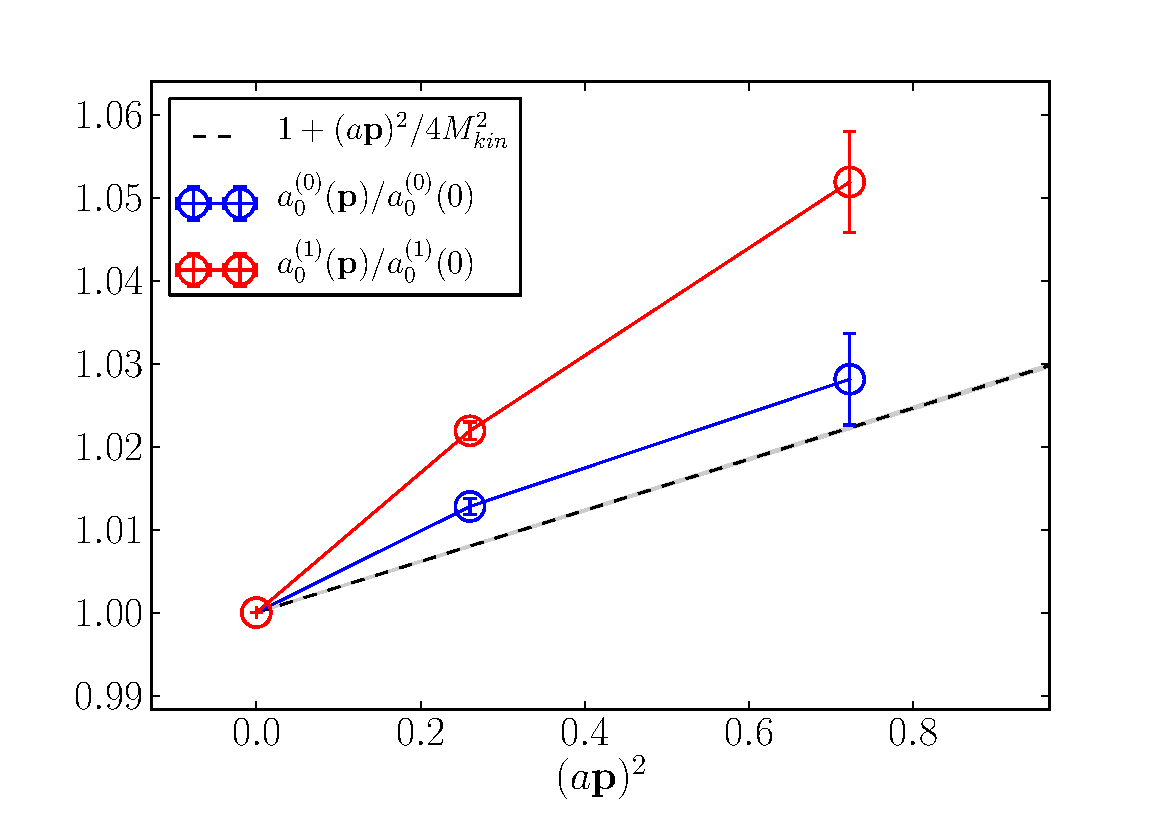
\includegraphics[width=0.85\textwidth]{images/nrqcd/relativistic_normalization_J0J1.pdf}
  \end{center}
  \caption{Decay amplitude ratios (colourful points) against the expected relativistic behaviour (grey dotted line and band). Adding the $A_{0,\text{lat}}^{(1)}$ piece of the current does not improve the relativistic behaviour of the ratio. \label{fig:relativisticnorm}}
\end{figure}

We gradually add corrections to this ratio by replacing $a_0^{0,0}$ with
\begin{align}
  \nonumber
  \label{eq:a_0corrections}
  a_0^{(0)}({\textbf{p}}) \sqrt{2E_{B_c}({\textbf{p}})} \,=\, \langle \Omega |& A_{0,\text{lat}}^{(0)} | B_c  ({\textbf{p}}) \rangle\,, \\
  \nonumber
  a_0^{(1)}({\textbf{p}}) \sqrt{2E_{B_c}({\textbf{p}})} \,=\, \langle \Omega |& (1+z^{A_0}_0 \alpha_s ) \left[A_{0,\text{lat}}^{(0)} +  A_{0,\text{lat}}^{(1)} \right] | B_c({\textbf{p}}) \rangle\,, \\
  \nonumber
  a_0^{(2)}({\textbf{p}}) \sqrt{2E_{B_c}({\textbf{p}})} \,=\, \langle \Omega |& \big[ (1+z^{A_0}_0 \alpha_s ) A_{0,\text{lat}}^{(0)} + (1 + z^{A_0}_1\alpha_s) A_{0,\text{lat}}^{(1)} \\ &+ z^{A_0}_2\alpha_s A_{0,\text{lat}}^{(2)}  \big] | B_c({\textbf{p}})\rangle\,.
\end{align}
we have here set the $\alpha=0,n$ superscripts implicit to make room for the new superscripts. The lattice currents $A_{0,\text{lat}}^{(n)}$ are those defined in Eq. \eqref{eq:nrqcd-hisq-current} for the temporal axial vector case. $a_0^{(0)}$ recreates the $A_0$ current to leading order in $\alpha_s$ and $1/m_b$, $a_0^{(1)}$ recreates $A_0$ up to order $\mathcal{O}(\alpha_s^2, \,(\Lambda_{\text{QCD}}/m_b)^2,\, ({\textbf{p}}/m_b)^2,\,\,\alpha_s \Lambda_{\text{QCD}} / m_b,\, \alpha_s {\textbf{p}}/m_b )$, and $a_0^{(2)}$ is up to order $\mathcal{O}( \alpha_s^2, (\Lambda_{\text{QCD}}/m_b)^2, ({\textbf{p}}/m_b)^2 )$.

Since the $z_0^{A_0}$ value is immediately avaliable from \cite{Monahan:2012dq}, we can show the result of taking the ratio $a_0^{(1)}({\textbf{p}})/a_0^{(1)}(0)$ as the red line in Fig. \ref{fig:relativisticnorm}. As can be seen, this pushes the ratio in the wrong direction, away from the relativistic dispersion relation line.

  We can determine values for $\left(z_1^{A_0}-z_0^{A_0}\right)$ and $\left(z_2^{A_0}-z_0^{A_0}\right)$ by demanding that $a^{(2)}_0({\textbf{p}})/a^{(2)}_0(0) = 1 + {\textbf{p}}^2/4M_{\text{kin}}^2$. Then, using the known $z_0^{A_0}$ values from perturbative matching we find
  \begin{align}
    z_1^{A_0} = -3.746267(95),\quad\quad z_2^{A_0} = -0.0002429(95).
  \end{align}
  $z_1^{A_0}$ here is required to be unnaturally large to overcome the suppression of $\alpha_s$ and drag the ratio downwards. 

The above analysis shows that the truncation of NRQCD-HISQ temporal-axial current used in current calculations is not sufficient to create a meson obeying a relativistic dispersion relation. This is perhaps indicative that further orders in the expansion are in fact important and should be included in lattice calculations. 

%% \subsubsection{Operator Matching}

%% In \cite{Morningstar:1997ep}, it is shown that this operator for the axial current by itself on the lattice is not totally sufficient to represent a continuum axial current. 
%% In this paper, the axial vector current with 1-loop corrections in continuum QCD (illustrated in figure 1, 2 and 3 in \cite{Morningstar:1997ep}) was computed using the on-shell mass and wave function renormalisation scheme in Feynman gauge. The light quark on-shell mass was approximated to zero, and the result was expanded in powers of the inverse heavy quark on-shell mass $1/M$.
%% \begin{align}
%% 	\nonumber
%% 	\langle q(p') | A_0 | h(p) \rangle_{\text{QCD}} = & \eta_1 [ \bar{u}_q(p') \gamma_5\gamma_0 u_h(p) ] + \eta_2 \left[ {p_0\over M} \bar{u}_h(p') \gamma_5 u_h(p) \right] \\
%% 	\nonumber
%% 	+ & \eta_3\left[ {p\cdot p'\over M^2} \bar{u}_q (p') \gamma_5\gamma_0 u_h(p)\right]
%% 	 + \eta_4\left[{p_0'\over M} \bar{u}_q(p') \gamma_5 u_h(p)\right] \\
%% 	 + & \mathcal{O}\left({1\over M^3}\right) \\ \nonumber \\
%% 	 \nonumber
%% 	 \eta_1 =  1 + &{\alpha_s\over 3\pi}\left[ 3\ln {M\over \lambda} - {11\over4} \right] \quad,\quad \eta_2 = {\alpha_s\over 3\pi} 2 \\
%% 	 \nonumber
%% 	 \eta_3 = {\alpha_s\over 3\pi} &\left[ 6\ln {M\over\lambda} - {8\pi\over 3}{M\over\lambda} + {1\over 2} \right] \quad,\quad \eta_4 = {\alpha_s\over 3\pi} \left[ -2 \ln {M\over \lambda} + {1\over 2} \right]
%% 	 \label{eq:continuum_axial}
%% \end{align}
%% $\lambda$ is the artificial Gluon mass (should cancel in obeservables), $|q(p')\rangle$ and $|h(p)\rangle$ are asymptotic light and heavy quark states respectively, and $u_{q,h}$ are the corresponding fermion wavefunctions. 

%% The dimensional requirements that $1/M$ must always come with a power of momenta turns this $1/M$ expansion into an expansion in velocity $v$, so is an NRQCD expansion. There are two expansions at play: $v$ and $\alpha_s$, one should avoid mixing them up.

%% In our lattice simulation the heavy quark obeys NRQCD so only has 2 components (there is no antiparticle without a relativistic dispersion relation). The particle and antiparticle fields in $h(x)$ can be decoupled using the Fouldy-Wouthuysen (FW) transformation \cite{Foldy:1949wa}, which is a canonical transformation, i.e. a change of variables of $h(x)$'s spinor degrees of freedom. Using the FW transformation, one can relate the $u_h$ to the wavefunction of a 2 component quark $U_h(p)$:
%% \begin{align}
%% 	u_h(p) = \exp\left(-{\underline{\gamma}\cdot{\textbf{p}}\over 2M}\right) \binom{U_h(p)}{0}
%% %	\label{eq:FW}
%% \end{align}
%% Using this to replace $u_h$ with $U_h$ in \eqref{eq:continuum_axial}, and inspecting the form of the leading order contributions, one can identify operators in the lattice theory that should be used to reproduce the continuum axial current $A_0$ \cite{Dowdall:2013tga}:
%% \begin{align}
%% 	&A_0 = (1+z_0 \alpha_s ) \left[ A_{0,\text{lat}}^{(0)} + (1 + z_1\alpha_s) A_{0,\text{lat}}^{(1)} + z_2\alpha_s A_{0,\text{lat}}^{(2)} \right]
%% 	\label{eq:current_corrections}
%% \\	&A_{0,\text{lat}}^{(0)} = \bar{c} \gamma_5 \gamma_0 b
%% 	\nonumber
%% \\	&A_{0,\text{lat}}^{(1)} = -{1\over2m_b} \bar{c} \gamma_5 \gamma_0 \underline{\gamma}\cdot\underline{\nabla} b
%% 	\nonumber
%% \\	&A_{0,\text{lat}}^{(2)} = -{1\over2m_b} \bar{c} \underline{\gamma}\cdot\underline{\overleftarrow{\nabla}} \gamma_5 \gamma_0  b.
%% 	\nonumber
%% \end{align}
%% $c$ and $b$ are the quark creation operators. The mass $M$ has been replaced with the bare $b$ mass $m_b$, since the on-shell mass only exists in perturbation theory so has no meaning in terms of the lattice. 
%% The coefficients $\{z_i\}$ can be obtained from matching terms between continuum and lattice perturbation theory.

%% The values $\{z\}$ are not yet known for the $bc$ current, but to give an idea of order or magnitude, in fig. \ref{fig:relativistic} uses values from the temporal axial current between light and $b$ quarks. Taken from \cite{Dowdall:2013tga}, these are $z_0=-0.007(2)$, $z_1=-0.031(4)$, $z_2=-0.325(4)$. $\alpha_s = 0.267$ is taken from set 7 of \cite{Colquhoun:2015oha}, obtained from running down of $\alpha_s^{\overline{MS}}(M_Z)$ down to scales of the simulation dictated by $a$.

%% $A_{0,\text{lat}}^{(0)}$ is the naive current operator used before (i.e with local smearing $\tilde{B}_c = A_{0,\text{lat}}^{(0)}$ in \eqref{eq:correlator}). 
%% To calculate the corrections, 
%% this was replaced with $A_{0,\text{lat}}^{(1,2)}$, and the calculation and fitting was repeated to extract $a_0$, this time coenciding with 
%% $\langle 0 | A_{0,\text{lat}}^{(1,2)} | B_c({\textbf{p}}) \rangle$. From these values one can build up a better estimation to the continuum current 
%% $\langle 0 | A_0 | B_c({\textbf{p}}) \rangle$. In fig. \ref{fig:relativistic} we gradually add corrections to see the effect each has, defining
%% \begin{align}
%%   \nonumber
%%   \label{eq:a_0corrections}
%%   &a_0^{(0)} = \langle 0 | (1+z_0 \alpha_s ) A_{0,\text{lat}}^{(0)} | B_c({\textbf{p}}) \rangle \\
%%   &a_0^{(1)} = \langle 0 | (1+z_0 \alpha_s ) \left[ A_{0,\text{lat}}^{(0)} + (1 + z_1\alpha_s) A_{0,\text{lat}}^{(1)} \right] | B_c({\textbf{p}}) \rangle \\
%%   \nonumber
%%   &a_0^{(2)} = \langle 0 | (1+z_0 \alpha_s ) \left[ A_{0,\text{lat}}^{(0)} + (1 + z_1\alpha_s) A_{0,\text{lat}}^{(1)} + z_2\alpha_s A_{0,\text{lat}}^{(2)} \right] | B_c({\textbf{p}}) \rangle \\
%%   \nonumber
%% \end{align}

%% \begin{table}
%% \begin{center}
%%  \begin{tabular}{||c c c c c c c c c||} 
%%  \hline
%%  set & $(a{\textbf{p}})^2$ & $a\delta E_0({\textbf{p}})$  & $aM_{B_c}$ & $a_0^{(0)}({\textbf{p}})/a_0^{(0)}(0)$ & $a_0^{(1)}({\textbf{p}})/a_0^{(1)}(0)$ 
%%  & $a_0^{(2)}({\textbf{p}})/a_0^{(2)}(0)$ \\ [0.5ex] 
%%  \hline\hline
%%  1 & 0.02891 & 0.00537(23) & 2.61(11) & 1.0036(19) & 1.0046(21) & 1.0045(21) \\ \hline
%%  2 & 0.26023 & 0.04580(24) & 2.838(27) & 1.0164(23) & 1.0253(26) & 1.0251(26) \\ \hline
%%  3 & 0.72287 & 0.12456(46) & 2.823(14) & 1.0371(46) & 1.0615(50) & 1.0608(51) \\ \hline
%%  4 & 1.04093 & 0.17772(86) & 2.840(15) & 1.053(10) & 1.088(11) & 1.086(11) \\ [1ex] 
%%  \hline
%% \end{tabular}
%% \end{center}
%% \caption{Results from fits with varying momenta. The third column gives the kinetic mass deduced from $\delta E({\textbf{p}})$ for each ${\textbf{p}}$. using \eqref{eq:kinetic_mass}\label{tab:from_fit}}
%% \end{table}

%% \subsubsection{$A_0^{(3)}$ contribution}

%% These current corrections are only to $\mathcal{O}({\textbf{p}}_b/m_b)$, but $\sqrt{E^r_{B_c}/M_{B_c}}$ has it's leading behaviour in $\mathcal{O}({\textbf{p}}^2/M_{B_c}^2)$. This implies one needs to carry on the expansion of current corrections further, to $\mathcal{O}(1/m_b^2)$. The dominant term at this order arises at tree level from the first term in \eqref{eq:continuum_axial}, and the second term in a $1/M$ expansion of \eqref{eq:FW}. The corresponding lattice operator is
%% \begin{align}
%% 	A^{(3)}_{0,\text{lat}} = {1\over 8m_b^2} \bar{c} \gamma_5\gamma_0 \underline{\nabla}^2 b. 
%% \end{align}
%% This was computed in a lattice calculation and combined with the lower orders to produce $a^{(3)}_0 = a_0^{(2)} + A^{(3)}_{0,\text{lat}}$. In this case we set $\alpha_s = 0$ to just focus on tree level. The results are shown on fig. \ref{fig:A3}.
%% \begin{figure}
%% \begin{center}
%%     \begin{tikzpicture}
%%         \begin{axis} [width=14cm,height=9cm,
%%             xmin=-0.1,xmax=0.9,ymin=0.99,ymax=1.09,
%%             xlabel = $(a{\textbf{p}})^2$,
%%             legend pos=north west]

%%             \addplot[color=green, dashed]{ sqrt( sqrt( x + 2.834*2.834 )/2.834) };
%%             \addlegendentry{$\sqrt{E_{B_c}/M_{B_c}}$}

%%             \addplot+[color=blue, mark=*,
%%                     error bars/.cd,x dir=both, x explicit,  y dir=both, y explicit]
%%                 coordinates {
%%                 		(  0.0 ,  1.0  ) +- ( 0.0,  1.33226762955e-19  )
%% 		  	(  0.0289148446127 ,  1.00549267643  ) +- ( 0.0,  0.00176452228481  )
%% 			(  0.260233601514 ,  1.01836440302  ) +- ( 0.0,  0.00222088535291  )
%% 			(  0.722871115317 ,  1.0390590324  ) +- ( 0.0,  0.00452197676768  )
%%             };
%%             \addlegendentry{$a_0^{(0)}({\textbf{p}})/a_0^{(0)}(0)$}

%%             \addplot+[color=red, mark=*,
%%                     error bars/.cd,x dir=both, x explicit,  y dir=both, y explicit]
%%                 coordinates {
%%                 		(  0.0 ,  1.0  ) +- ( 0.0,  0.0  )
%%           	        (  0.0289148446127 ,  1.00663334793  ) +- ( 0.0,  0.00194538583335  )
%% 			(  0.260233601514 ,  1.02734203998  ) +- ( 0.0,  0.00244820981549  )
%% 			(  0.722871115317 ,  1.06347584999  ) +- ( 0.0,  0.00497690081001  )
%%             };
%%             \addlegendentry{$a_0^{(1)}({\textbf{p}})/a_0^{(1)}(0)$}
            
%%             \addplot+[color=orange, mark=*,
%%                     error bars/.cd,x dir=both, x explicit,  y dir=both, y explicit]
%%                 coordinates {
%%                 		(  0.0 ,  1.0  ) +- ( 0.0,  0.0  )
%% 			(  0.260233601514 ,  1.0211157939  ) +- ( 0.0,  0.00302333986783  )
%% 			(  0.722871115317 ,  1.05858288737  ) +- ( 0.0,  0.00568371480017  )
%%             };
%%             \addlegendentry{$a_0^{(3)}({\textbf{p}})/a_0^{(3)}(0)$}

%%         \end{axis}
%%     \end{tikzpicture}
%% \end{center}
%% \caption{Relativistic Normalisation of 1-loop corrected Axial Current. $a_0^{(n)}$ are defined in \eqref{eq:a_0corrections}. (tree level) }
%% \label{fig:A3}
%% \end{figure}
%% As a sanity check for the $A^{(3)}$ calculation, fig. \ref{fig:A3A2} shows the ratio $A^{(3)}_{0,\text{lat}}({\textbf{p}})/A^{(2,1)}_{0,\text{lat}}({\textbf{p}})$. Since $A^{(3)} = \mathcal{O}({\textbf{p}}^2)$ and $A^{(1)} = \mathcal{O}({\textbf{p}})$, we expect such a ratio to be proportional to $|{\textbf{p}}|$ (see fig. \ref{fig:A3A1}). {\color{red}{The $A^{(3)}/A^{(2)}$ line isn't straight...}}

%% %==========
%% \begin{figure}
%% \begin{center}
%%     \begin{tikzpicture}
%%         \begin{axis} [width=14cm,height=9cm,
%%             xlabel = $a|{\textbf{p}}|$,
%%             legend pos=north west]

%%             \addplot+[color=red, mark=*,
%%                     error bars/.cd,x dir=both, x explicit,  y dir=both, y explicit]
%%                 coordinates {
%%                		(  0.0 ,  0.168061897514  ) +- ( 0.0,  0.00761364082979  )
%% 			(  0.510130965061 ,  0.255812358549  ) +- ( 0.0,  0.0171547894616  )
%% 			(  0.850218275102 ,  0.291882276843  ) +- ( 0.0,  0.0323767757253  )
                    
%%             };
%% \addlegendentry{$A^{(3)}_{0,\text{lat}}({\textbf{p}})/A^{(1)}_{0,\text{lat}}({\textbf{p}})$}

%%         \end{axis}
%%     \end{tikzpicture}
%% \end{center}
%% \label{fig:A3A1}
%% \caption{Ratio of third current correction to first.}
%% \end{figure} 

\section{$B_{(s)}\to D_{(s)}l\nu$ form factors}
\label{sec:BD_BsDs_nrqcd}

I attempted a calculation of the $B\to Dl\nu$ and $B_{s}\to D_{s}l\nu$ form factors, $f_{0,+}(q^2)$ and $f^s_{0,+}(q^2)$, using the 2+1+1 MILC ensembles, HISQ $l$,$s$ and $c$ valence quarks, and an NRQCD valence $b$ quark. This study was similar to previous studies of $B\to Dl\nu$ form factors \cite{Na:2015kha} and $B_s\to D_sl\nu$ form factors \cite{Monahan:2017uby}. The main difference between this and the previous studies was that they used older MILC ensembles that do not take the charm into account in the sea.

This study was not completed on account of two major problems:
\begin{itemize}
  \item
    The $\order{\alpha_s{\textbf{p}}/m_b}$ terms in the vector NRQCD-HISQ current that we must ignore due to the lack of perturbative normalizations, $V_{k}^{(2)}$ and $V_{k}^{(4)}$, turned out to be significant in magnitude.
  \item
    On one ensemble in the $B_s\to D_s l\nu$ case, there was an anomalous result for the vector current matrix element extracted from the correlator fits.
\end{itemize}
We give an outline of the calculation here for completeness, but the crucial findings of this section are these two issues.

\subsection{Calculation Details}

\begin{table}[t!]
\hspace{-40pt}
 \begin{tabular}{c c c c c c c c c c c}
 \hline
 Set & handle & $am^{\text{val}}_{s0}$ & $am^{\text{val}}_{c0}$ & $am^{\text{val}}_{b0}$ & $u_0$ & $c_{1,6}$ & $c_5$ & $c_4$ & $\{T\}$ & $a_{\text{sm}}/a$ \\ [0.5ex] 
 \hline
 0 & {\textbf{very coarse}} & 0.0705 & 0.826 & 3.297 & 0.8195 & 1.36 & 1.21 & 1.22 & 8, 11, 14 & 0, 2.0, 4.0 \\ [1ex]
 1 & {\textbf{coarse}} & 0.0541 & 0.645 & 2.66 & 0.8340 & 1.31 & 1.16 & 1.20 & 9, 12, 15 & 0, 2.0, 4.0 \\ [1ex]
 2 & {\textbf{fine}} & 0.0376 & 0.450 & 1.91 & 0.8525 &  1.21 & 1.12 & 1.16 & 14, 19, 24 & 0, 3.425, 6.85 \\ [1ex]
 \hline
\end{tabular}
 \caption{Parameters used in our calculation. $am^{\text{val}}_{s0}$ and $am^{\text{val}}_{c0}$ are the bare masses of the strange and charm valence quarks, tuned in \cite{PhysRevD.91.054508}. $am^{\text{val}}_{b0}$ is the bare mass of the valence bottom quark, tuned in \cite{Dowdall:2011wh}. $u_0$ is the 'tadpole improvement parameter' as used in \cite{Dowdall:2011wh}. $\{c_i\}$ are the coefficients for the kinetic and chromomagnetic terms in the NRQCD action (Eq. \eqref{eq:nrqcd_dH}) \cite{Hammant:2013sca}. $\{T\}$ is the set of temporal seperations between source ($B_{(s)}$ creation operator) and sink ($D_{(s)}$ anihilation operator). $a_{\text{sm}}$ are the radii of the exponential smearing function applied to the $B_{(s)}$ and $D_{(s)}$ creation operators.
   \label{tab:quarkmasses}}
\end{table}

Correlation functions were generated on three MILC ensembles, sets 0, 1 and 2 in Table \ref{tab:ensembles}. When using the NRQCD action, one is limited to the coarser end of the spectrum of ensembles. This is because in the $a\to 0$ limit subleading terms in $\delta H$ (eq. \eqref{eq:nrqcd_dH}) and $J^{(n>0)}_{\mu}$ (eq. \eqref{eq:nrqcd-hisq-current}) diverge, since the $1/m_b$ factors are infact proportional to $1/am_b$, resulting negative powers of the lattice spacing. However, NRQCD discretisation effects are small relative to other discretizations due to the lack of the $b$ rest mass, so we can afford to use coarser lattices. Also, obviously, using coarse lattices means the project is computationally inexpensive. The bare parameters used to generate the correlation functions are shown in table \ref{tab:quarkmasses}.

We generated 2-point correlation functions for $B_{(s)}$ and $D_{(s)}$ mesons, and 3-point correlators between $B_{(s)}$ and $D_{(s)}$ interpolating operators with $V^{(n)}_{\mu}$ currents inserted for all $\mu$ and $n=0,1,2$($\mu=0$) and $n=0,1,2,3,4$($\mu=1,2,3$). For the $B_{(s)}$ operator we use exponential smearing functions (like those introduced in Eq. \eqref{eq:smearings}), smearing radii $a_{\text{sm}}$ are given in Table \ref{tab:quarkmasses}.

The $B_{(s)}$ 2-point correlators, $C_{B_{(s)}}^{\alpha\beta}(t)$ were generated using Eq. \eqref{eq:nrqcd-hisq-2pt}, with the charm propagator replaced with a strange or light propagator, and $\mathcal{O}_{m} = \gamma_0\gamma_5$. We also computed $D_{(s)}$ 2-point correlators at a number of spacial momenta $\{{\textbf{p}}\}$ (given in Table \ref{tab:nrqcd_twists}), generated by
\begin{align}
  C_{D_{(s)}}^{\alpha\beta}({\textbf{p}},t) = \sum_{{\textbf{x}},{\textbf{x}}'}\sum_{{\textbf{y}},{\textbf{y}}'} \phi^{\alpha}({\textbf{x}}-{\textbf{x}}')\phi^{\beta}({\textbf{y}}-{\textbf{y}}') \left\langle \text{Tr}_c[g_c^{\theta_{\textbf{p}}}({\textbf{x}},t,{\textbf{y}};t_0) g^{\dagger}_{l(s)}({\textbf{x}}',t;{\textbf{y}}',t_0) ]\right\rangle,
\end{align}
where $\phi^{\alpha}({\textbf{x}})$ are the smearing functions (Eq. \eqref{eq:smearings}), $g_{l(s)}$ are light or strange staggered propagators, and $g_c^{\theta_{\textbf{p}}}$ is a charm staggered propagator with momentum twist $\theta_{\textbf{p}}$. Tr$_c$ is over color.

We generated 3-point correlators for each individual piece of the NRQCD-HISQ current, and each {\textbf{p}}, using
\begin{align}
  %% C_{V_{\mu}^{(n)}}^{\alpha\beta} ({\textbf{p}},t,T) = \sum_{\textbf{x},\textbf{y},\textbf{z}} \left\langle \text{Tr}_c\left( g_c^{\theta_{\textbf{p}}}(x,y) g_{l(s)}^{\dagger}(x,z) \text{Tr}_s\left[ \gamma_0 \Omega(x)\Omega(y) \mathcal{O}_{n,\mu}G_b(y,z) \gamma_z \right] \right) \right\rangle.
  C_{V_{\mu}^{(n)}}^{\alpha\beta} &({\textbf{p}},t,T) = \sum_{\textbf{x},\textbf{y},\textbf{z}} (-1)^{\sum_{k=1}^3 x_k/a} \,\,\phi^{\alpha}({\textbf{x}}-{\textbf{x}}') \phi^{\beta}({\textbf{z}}-{\textbf{z}}')\times \\ \nonumber &\left\langle \text{Tr}_c\left( g_c^{\theta_{\textbf{p}}}({\textbf{x}},t_0;{\textbf{y}},t) g_{l(s)}^{\dagger}({\textbf{x}},t_0;{\textbf{z}},T) \text{Tr}_s\left[ \gamma_0 \Omega^{\dagger}({\textbf{y}},t) \mathcal{O}_{n,\mu}G_b({\textbf{y}},t;{\textbf{z}},T) \Omega({\textbf{z}},T)\gamma_0 \right] \right) \right\rangle.
\end{align}
$\mathcal{O}_{n,\mu}$ are defined by $J_{\mu}^{(n)} = \bar{\psi}_c \mathcal{O}_{n,\mu} \Psi_b$, where $J_{\mu}^{(n)}$ are pieces of the NRQCD-HISQ vector current (Eq. \eqref{eq:nrqcd-hisq-current}).

The list of twists we used on each ensemble is given in table \ref{tab:nrqcd_twists}. Due to the signal/noise degradation of the $D_{(s)}$ correlators as one adds more spacial momentum, our lattice data was limited to the high $q^2$ region. One motivation for this study was to test how far down the $q^2$ range we could reach with lattice data before the noise in the correlators made the data useless.

\begin{table}[htb!]
  \vspace{10pt}
  \hspace{-20pt}
 \begin{tabular}{c c c c c}
 \hline
 & Set & $\theta$ & $|a{\textbf{p}}|$ & $q^2$[GeV$^2$] \\ [0.5ex] 
 \hline
 $B\to D$ & 0 & 0, 0.74, 1.47, 2.20, 2.94 & 0, 0.25, 0.5, 0.75, 1.00 & 11.8, 11.6, 10.8, 9.4, 7.3 \\ [1ex]
 & 1 & 0, 1.58, 2.24, 4.53 & 0, 0.36, 0.51, 1.02 & 11.8, 10.8, 9.9, 5.0  \\ [1ex]
 & 2 & 0, 1.76, 2.64 & 0, 0.30, 0.49 & 11.8, 10.7, 9.3 \\ [1ex]
 \hline
 $B_s\to D_s$ & 0 & 0, 0.74, 1.47, 2.20, 2.94 & 0, 0.25, 0.5, 0.75, 1.03 & 11.8, 11.6, 10.9, 9.5, 7.6 \\ [1ex]
 & 1 & 0, 1.10, 2.20, 3.31, 4.41 & 0, 0.25, 0.50, 0.75, 1.00 & 11.8, 11.3, 10.1, 8.1, 5.7 \\ [1ex]
 & 2 & 0 & 0 & 11.8\\  [1ex]
 \hline
\end{tabular}
 \caption{Momentum twists (and corresponding momenta and $q^2$ values) given to the charm propagator on each ensemble. \label{tab:nrqcd_twists} }
\end{table}

\subsection{Correlator Fits}

We extract current matrix elements from the generated correlation functions, via simultaneous Bayesian fits as described in Sec. \ref{sec:correlator_fits}. For the set of 2-point correlators we use Eq. \eqref{eq:2ptfit_wsmears} (with $n=m=0$), and 3-point correlators are fit to
\begin{align}
  \nonumber
  C^{\alpha\beta}_{3}(t,T)|_{\text{fit}} =& \sum_{j,k=0}^{N_{\text{exp}},N_{\text{exp}}} \Big(\, a^{B_{(s)}}_j J^{nn}_{jk} a^{D_{(s)}}_k f(E^{B_{(s)}},t) f(E^{D_{(s)}}_n,T-t)
  \\ \nonumber
  &+a^{B_{(s)},o}_{\alpha,j} J^{on}_{jk} a_{\beta,k}^{D_{(s)}} (-1)^t f(E^{B_{(s)},o}_n,t) f(E^{D_{(s)}},T-t)
  \\ \nonumber
  &+a_{\alpha,j}^{B_{(s)}} J^{no}_{jk} a_{\beta,k}^{D_{(s)},o} (-1)^{T-t} f(E^{B_{(s)}},t) f(E^{M'^*,o}_n,T-t)
  \\
  &+a_{\alpha,j}^{B_{(s)},o} J^{oo}_{jk} a_{\beta,k}^{D_{(s)},o} (-1)^T f(E^{B_{(s)},o}_n,t) f(E^{D_{(s)},o},T-t) \,\Big).
  \label{eq:3ptcorrelator_real}
\end{align}
We set $N_{\text{exp}}=5$ in each fit. We performed a single simultanious fit containing each correlator computed for each ensemble, taking into account correlations between all time slices of all correlation functions involved in the fit.

We set gaussian priors for the parameters $J_{jk}$, and log-normal priors for most other parameters. Using log-normal distributions ensures energies $E_n^M$ and amplitudes $a_n^M$ are positive and forbids them from moving arbitrarily close to zero, improving the stability of the fit. The exception is the smeared amplitudes $a^{\alpha>0}_n$, which can be zero or negative, so we simply set gaussian priors for these.

Priors for the ground state energies and amplitudes (oscillating and non-oscillating) are set via an empirical Bayes approach. Plots of effective masses and amplitudes are inspected to find reasonable central values of priors (see Sec. \ref{sec:BsDsstar_fits} for definitions of effective masses and amplitudes). A generic variance of 10\% of the central value is given in all cases. The typical precision of fit results for these parameters is of order 0.1\%, much more precise than their priors. The log of the all excited state energies are given generic priors log$(\Lambda_{\text{QCD}}\pm\Lambda_{\text{QCD}}/2)$, where we set $\Lambda_{\text{QCD}}=0.5$GeV. The log of the excited state (non-smeared) amplitudes are set to $log(0.3\pm 0.2)$. The smeared exicted state amplitudes are given priors of  $0.3\pm 0.2$. All 3-point transition parameters $J_{jk}$ are given priors of $0\pm 1$.

We typically set $t_{\text{cut}}=3$ for 2- and 3-point correlators in the fit on the fine ensemble (set 2) and $t_{\text{cut}}=2$ on very coarse and coarse (sets 0 and 1). For some specific correlators, a larger $t_{\text{cut}}$ is necessary to acheive a good fit ($\chi^2/N_{\text{dof}} < 1$), these higher $t_{\text{cut}}$ values are always in the range $t_{\text{cut}}\in[2,8]$. An svd-cut is applied in each fit, with a specific choice of cut determined according to what acheives a good fit. The svd-cut is typically of the order $10^{-3}$.

The current matrix element we require to find $h_{A_1}^s(1)$ is given by
\begin{align}
  \langle D_s | V_{\mu}^{(n)} | B_s \rangle |_{\text{lat}} = 2 \sqrt{M_{B_s}E_{D_s}} J^{nn}_{00}.
  \label{eq:currentfit}
\end{align}

\subsection{Form Factors}

We construct 'continuum' vector currents $\langle D_{(s)}| V_{\mu} | B_{(s)} \rangle \equiv \langle V_{\mu} \rangle$ from the lattice expectation values $\langle D_{(s)} | V_{\mu}^{(n)} | B_{(s)} \rangle |_{\text{lat}}$ according to Eq. \eqref{eq:nrqcd-hisq-current-truncate}, i.e. only including the first two current pieces $V^{(0)}_{\mu}$ and $V^{(1)}_{\mu}$. We also compute $V^{(2)}_{0}$ and $V^{(2,3,4)}_k$ to assess their size and the validity of ignoring them, this is adressed in Sec. \ref{sec:largesubleadingcurrents}.

We take the average over the spacial currents, resulting in two distinct current matrix elements $\langle V_0 \rangle$ and $\langle V_k \rangle$. Then, from the definition of pseudoscalar-pseudoscalar form factors (Eq. \eqref{eq:formfactors_experimental}), we find (defining $M_{B_{(s)}}\equiv M$, $M_{D_{(s)}}\equiv m$, $E_{D_{(s)}}\equiv E$, and ${\textbf{p}}_{D_{(s)}} \equiv {\textbf{p}}$)
\begin{align}
  \langle V_0 \rangle &= f^{(s)}_+(q^2) \left[ M + E - {M^2-m^2\over q^2}(M-E) \right] + f^{(s)}_0(q^2) {M^2-m^2\over q^2}(M-E), \\
  \langle V_k \rangle &= {|{\textbf{p}}|\over \sqrt{3}} \left[ f^{(s)}_+(q^2) \left( 1 + {M^2-m^2\over q^2} \right) - f^{(s)}_0(q^2) {M^2-m^2\over q^2} \right].
\end{align}
By inverting these relations we deduce $f^{(s)}_{0,+}(q^2)$ from $\langle V_0 \rangle$,$\langle V_k \rangle$ at the lattice spacings of each ensemble.

We aim then to extrapolate these form factors to $a=0$ and to all $q^2$. We did not obtain any lattice data at smaller light quark masses so cannot extrapolate to the physical light mass. In the $B_s\to D_sl\nu$ case, the size of such an effect is small (see chapters \ref{chap:BsDsstar} and \ref{chap:BsDs}). In the $B\to Dl\nu$ case, however, this could result in considerable uncontrolled systematic errors.

We parameterise the functional form of $f^{(s)}_{0,+}(q^2)$ using the BGL parameterization \cite{PhysRevD.79.013008}. This involves first defining the map
\begin{align}
	z(q^2) = {\sqrt{t_+ - q^2} - \sqrt{t_+ - t_0} \over \sqrt{t_+ - q^2} + \sqrt{t_+ - t_0} }\,,
\end{align}
where $t_{\pm} = (M_{B_{(s)}} \pm M_{D_{(s)}})^2$ and we choose $t_0 = t_+( 1 - \sqrt{1 - t_-/t_+})$, and . $z(q^2)$ has a very small magnitude throughout the entire $q^2$ range, in our case $|z| < 0.032 \,\,\forall \,\,$physical$\,q^2$. %It can be shown that $f_{0,+}^{(s)}(q^2)$ is analytic in the unit disc of the $z-$plane (see e.g. \cite{Hill:2006ub}).
$f^{(s)}_{+,0}(q^2)$ can be expressed as a series expansion in $z$:
\begin{align}
	f_{0,+}(q^2) = {1\over P_{0,+}(q^2)} \sum^K_{k=0} a^{0,+}_k z(q^2)^k.
	\label{eq:zexpansion}
\end{align}
we truncate this at $K=2$, adding further terms has no effect on the fit. The factors $P(q^2)$ are defined by
\begin{align}
	P_{0,+}(q^2) = \left( 1 - {q^2\over M_{0,+}^2}\right).
\end{align}
These are required due to subthreshold poles in the crossed channel of $\langle D_{(s)} | V_{\mu} | B_{(s)} \rangle$, which in our case is a $W$ decay into a $B^*_c$ meson. The pole is located where the $W$ has the correct momentum $q^2$ to create the $B_c$, hence at $q^2=M_{B^*_c}$. This is not within the $q^2$ range, but can create curvature in $f_{0,+}$ that can confound the expansion in $z$. $P_{0,+}$ effectively removes this pole from the $z$ expansion.

The discretisation effects in our form factors are controlled for by modifying \eqref{eq:zexpansion}:
\begin{align}
	a^{0,+}_n \to a^{0,+}_n \times ( 1 + b^{0,+}_n (am^{\text{val}}_{c0})^2 ),
\end{align}
where $b^{0,+}_n$ are new fit parameters. $am_c\to0$ in the continuum limit, and, since the charm mass is the largest scale involved in our calculation, it serves as a good order parameter for discretization effects. $\{a_n^{0,+},b_n^{0,+}\}$ are all given gaussian prior distributions of $0\pm 1$.

\subsection{Results}

%% \begin{figure}
%% \centering
%% \begin{subfigure}{.55\textwidth}
%%   \centering
%%   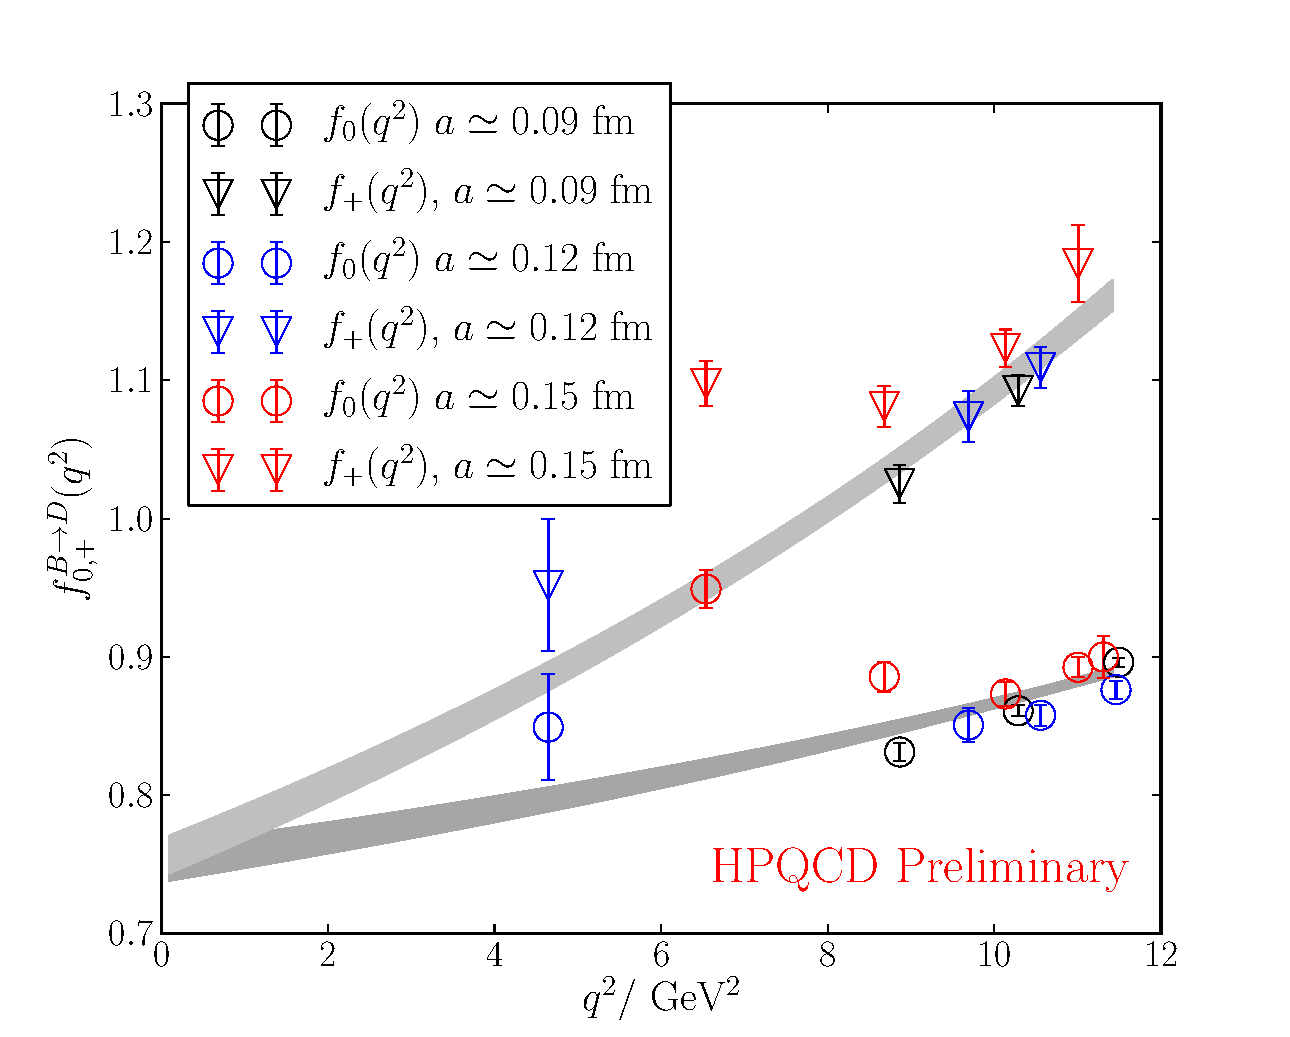
\includegraphics[width=1.0\linewidth]{images/NRQCD/BD_apr18.pdf}
%%   \label{fig:sub1}
%% \end{subfigure}%
%% \begin{subfigure}{.55\textwidth}
%%   \centering
%%   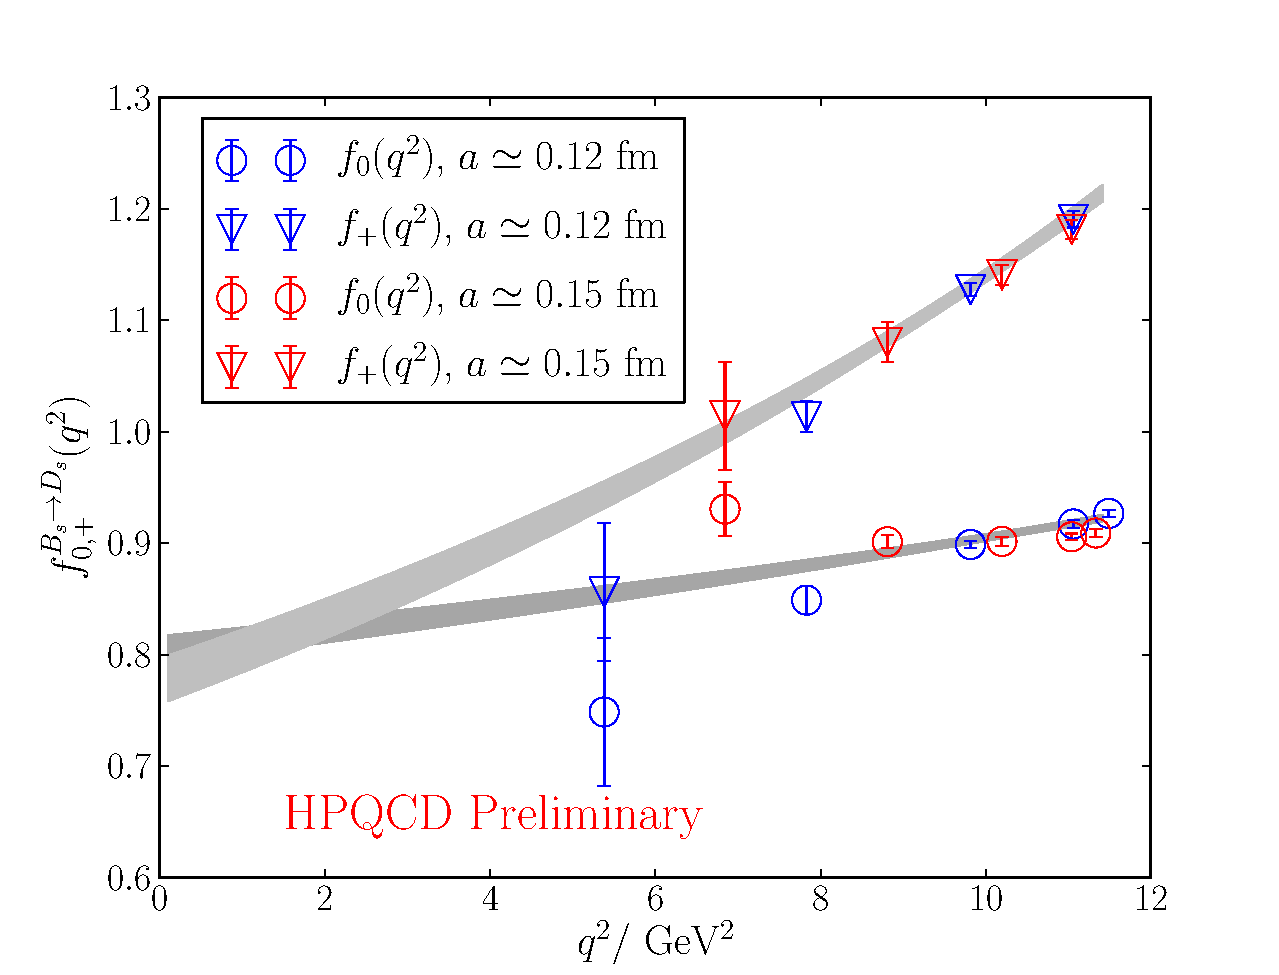
\includegraphics[width=1.0\linewidth]{images/NRQCD/BsDs_apr18.pdf}
%%   \label{fig:sub2}
%% \end{subfigure}
%% \caption{Left: $B\to D l\nu$ form factors from the NRQCD calculation. Right: $B_{(s)}\to D_{(s)} l\nu$ form factors using an identical approach. Errors are statistical. The bands give a kinematic extrapolation to all $q^2$, see second year report. The statistical errors grow as $q^2$ decreases due to Parisi-Lepage scaling (sec.9.3.2 of \cite{DeGrand:2006zz}).}
%% \label{fig:nrqcd}
%% \end{figure}

The extrapolation of our lattice data to all $q^2$ and $a=0$ is illustrated in Figures \ref{fig:BD_formfactors} and \ref{fig:BsDs_formfactors}. As can be seen here, statistical errors in the lattice data increase exponentially with momentum twist (as $q^2$ decreases). Besides this, the very coarse (and to an extent coarse) data suffers from large discretization effects as the twist is increased, pushing the results upwards.

\begin{figure}[htb!]
  \begin{center}
    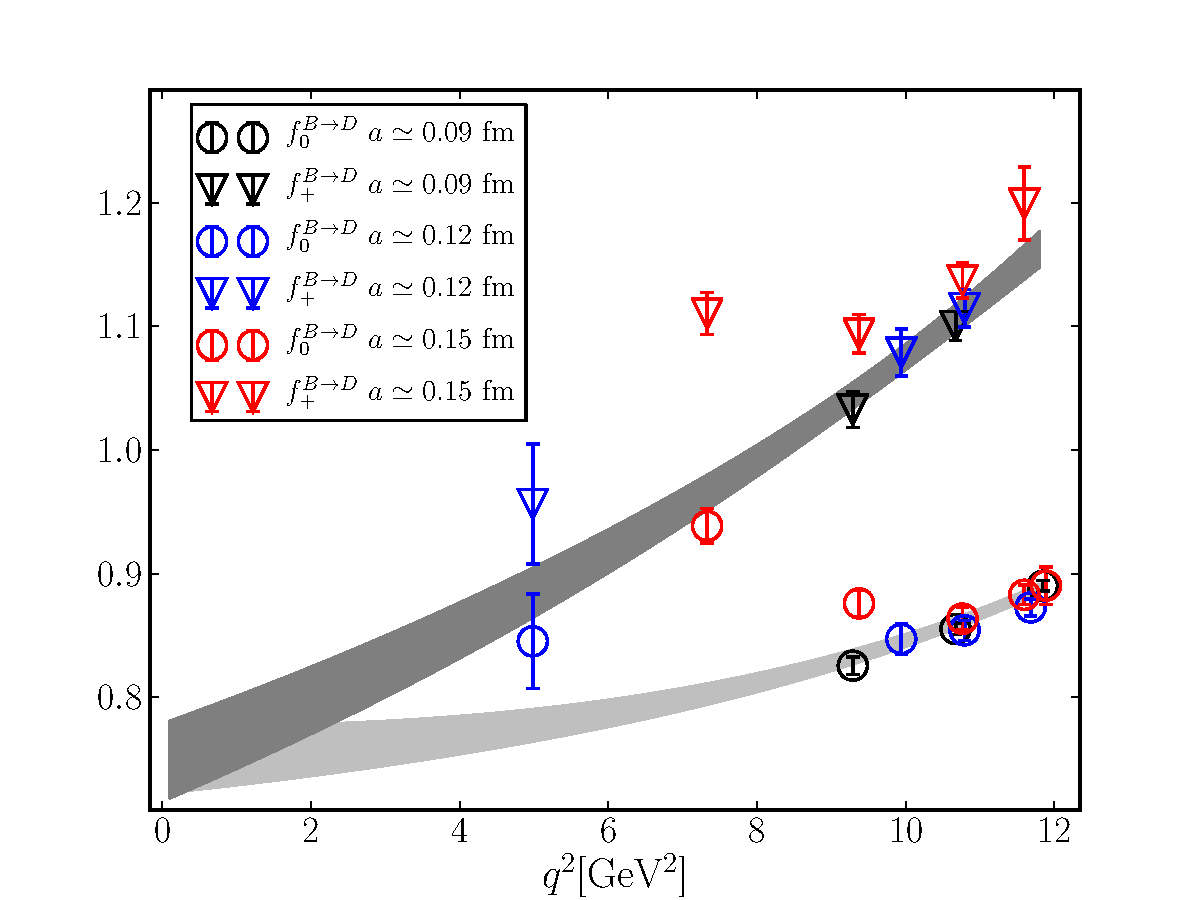
\includegraphics[width=0.85\textwidth]{images/nrqcd/BD_formfactors.pdf}
  \end{center}
  \caption{$B\to Dl\nu$ form factors. The coloured points show lattice data, each color represents an ensemble. The grey band represents the continuum and kinematically extrapolated result. \label{fig:BD_formfactors}}
\end{figure}

\begin{figure}[htb!]
  \begin{center}
    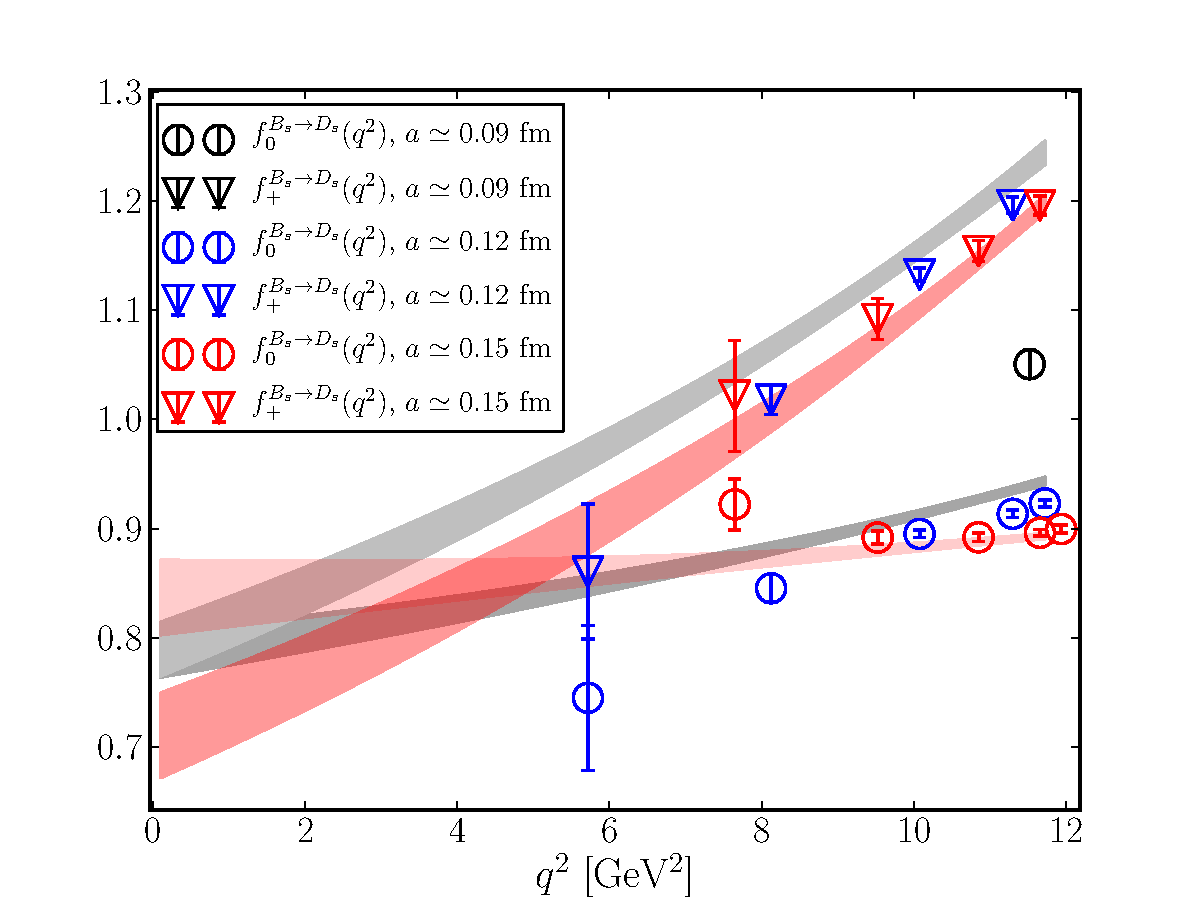
\includegraphics[width=0.85\textwidth]{images/nrqcd/BsDs_formfactors.pdf}
  \end{center}
  \caption{$B_s\to D_sl\nu$ form factors. The coloured points show lattice data, each color represents an ensemble. The grey band represents the continuum and kinematically extrapolated result. \label{fig:BsDs_formfactors}}
\end{figure}

I now go on to discuss the two issues which lead me to abandon this project.

\subsubsection{Anomalous Results}

In the $B_s\to D_s l\nu$ case I have not include lattice results from the fine ensemble in the $q^2$ and $a\to 0$ extrapolation. This is because the lattice results for $f_0^s(q^2)$ on this ensemble are clearly wrong. We have {\textit{a priori}} knowledge of what, for example, the ballpark of $f_0^s(q^2_{\text{max}})$ should be from a couple of sources:
\begin{itemize}
\item
The result should not vary much more than $\mathcal{O}(a^2)$ (where $a$ is the lattice spacing) from the same result on other ensembles.
\item
  The result should not vary much more than $\mathcal{O}(am^{\text{val}}_{s0} - am^{\text{val}}_{l0})$ from the same number on the same ensemble for the $B\to D$ calculation (Chiral symmetry).
\end{itemize}
However, we find the fits to $q^2_{\text{max}}$ data on the fine ensemble produce a result for $J^{nn}_{00}$ that is much larger than what is expected from these considerations. This is accompanied by the fits being very unstable, varying by a number of sigmas when different combinations of data are included, and different hyperparameters (svd-cut, $t_{\text{cut}}$, etc) are included. A number of tests have been carried out to find out exactly what is causing this issue, but no compelling evidence has emerged for any explanation. Fig. \ref{fig:BsDs_f0q2max} illustrates the situation.

It is worth keeping in mind that NRQCD results have no continuum limit since the action and the currents are truncated sums of inverse masses in lattice units, therefore the truncation error grows like $a^{-n}$ as $a\to 0$. What we are seeing here may be the result of large $1/(am_b)^2$ corrections to the NRQCD-HISQ current being ignored.

\begin{figure}[htb!]
  \vspace{-20pt}
  \begin{center}
    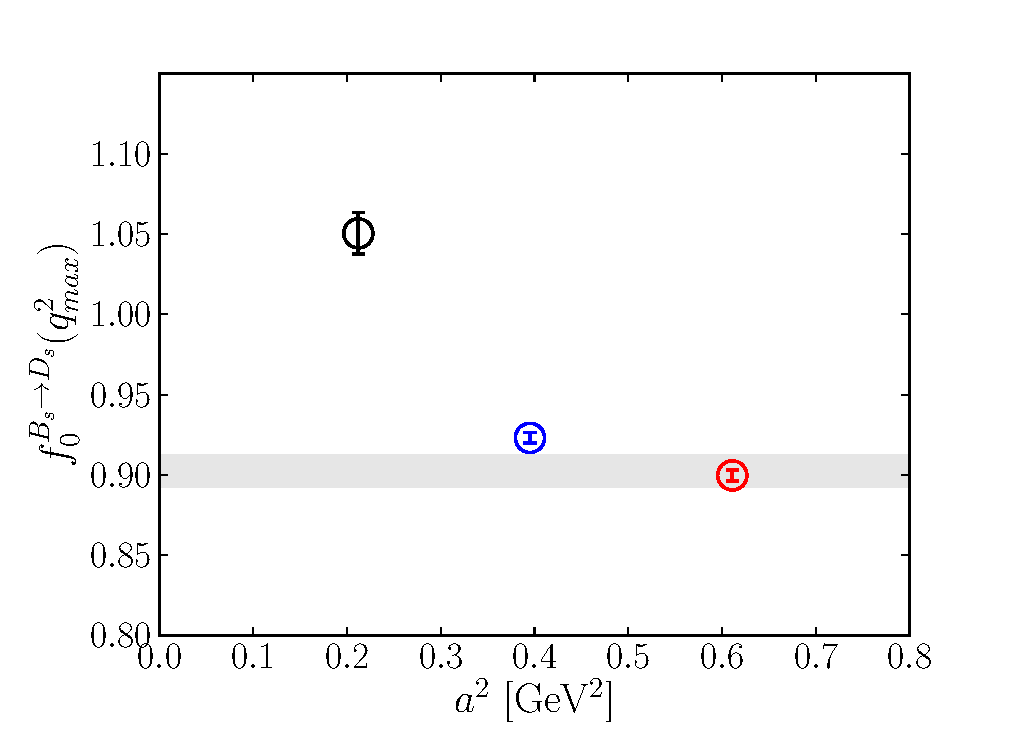
\includegraphics[width=0.75\textwidth]{images/nrqcd/BsDs_f0q2max.pdf}
  \end{center}
  \caption{Lattice results for $f_0^s(q^2_{\text{max}})$ against $a^2$. The grey band shows the result for $f_0^s(q^2_{\text{max}})$ computed in chapter \ref{chap:BsDs} using the Heavy-HISQ approach for comparison. Clearly the result on the fine ensemble (the black point), and possibly on the coarse ensemble (the blue point), contain large unknown systematic errors. \label{fig:BsDs_f0q2max}}

\end{figure}

\subsubsection{Large Subleading Currents}
\label{sec:largesubleadingcurrents}

Another problem that has uncovered itself in the NRQCD calculation is large subleading currents. Namely, the pieces $V^{(2,4)}_k$ of the spatial vector current. We determined these currents as part of the calculation in order to assess if they are suitably small such that they can be ignored. These turned out to have a magnitude $\sim 35\%$ of the leading order.

\begin{figure}[htb!]
  \begin{center}
    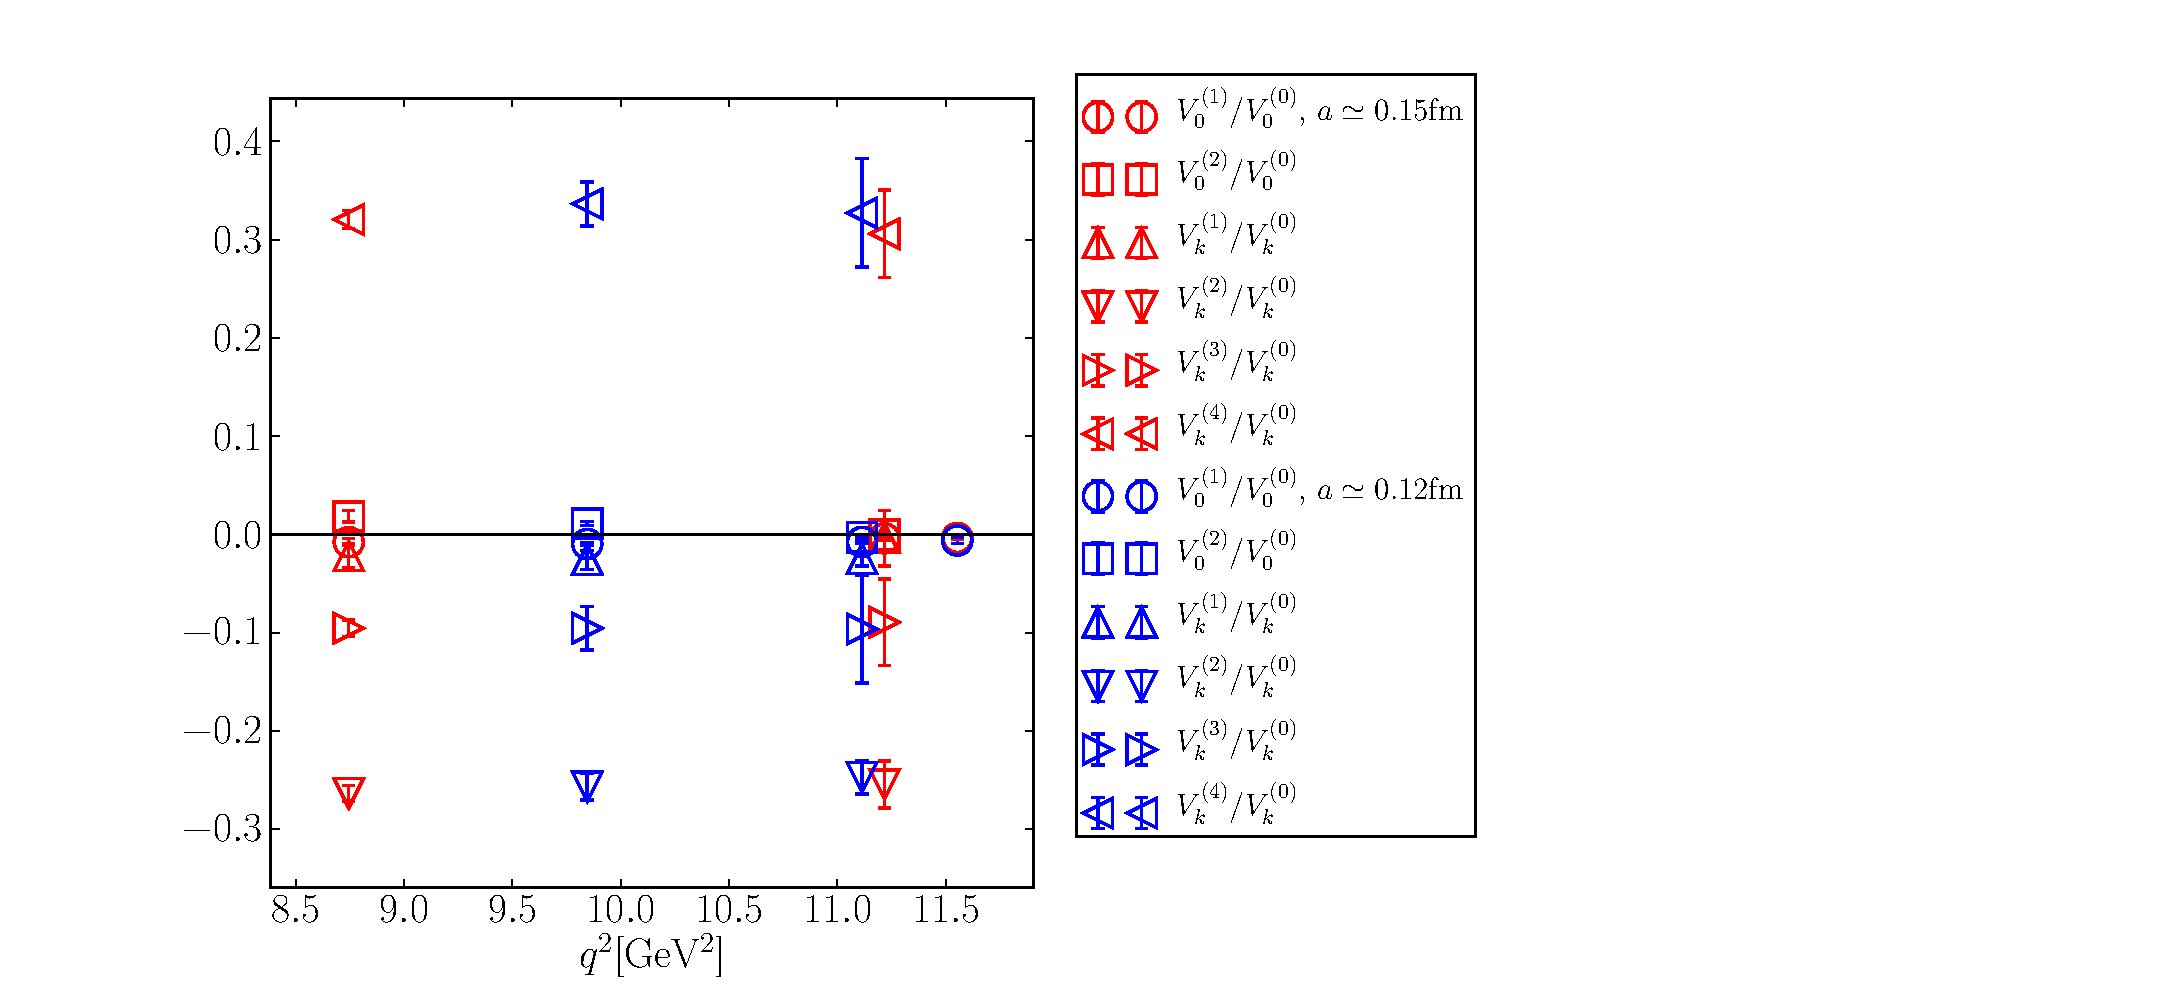
\includegraphics[width=1.2\textwidth]{images/nrqcd/BsDs_currentratios.pdf}
  \end{center}
  \caption{Ratios of (matrix elements of) the subleading NRQCD-HISQ currents $V_{\mu}^{(n>0)}$ to the leading order current $V_{\mu}^{(0)}$, in the $B_s\to D_s$ case. \label{eq:currentratios}}
\end{figure}

In Fig. \ref{eq:currentratios}, we show the ratios of (matrix elements of) NRQCD-HISQ currents in the $B_s\to D_s$ case. All ratios are between the subleading currents $V_{\mu}^{(n>0)}$ and the leading order current $V_{\mu}^{(0)}$, in order to show the size of the subleading currents relative to the leading order. $V^{(1)}_{\mu}$ is included in our result so we do not need to worry about its size. $V_0^{(2)}$ and $V_k^{(3)}$ are $\lessapprox 10\%$ of the leading order, given that these also receive $\order{\alpha_s}$ suppression, their negligence is relatively harmless.

$V_k^{(2,4)}$, however, have considerable magnitude. Neglecting them implies a naive systematic error of $\order{ 35\% \times \alpha_s } \sim 8\%$. This would prevent any results from our calculation from being anywhere near competitive. These two currents are of order $\alpha_s{\textbf{p}}/m_b$, so their magnitude would likely only increase as we move towards $q^2=0$.

Since the problematic current pieces are exclusively part of the spacial vector current, we could remove this problem if we did not rely on the spacial vector current for extracting the form factors. The next section shows our attempt at such an alternative approach.

\subsection{Form factors from $V_0$ and $S$ in $B_{(s)}\to D_{(s)}$}
\label{sec:fplus_divergence}

Instead of using $\langle V_0 \rangle$ and $\langle V_k \rangle$ to extract $f^{(s)}_{0,+}(q^2)$, one could in principle instead use the combination $\langle V_0 \rangle$ and $\langle S \rangle$, where $S$ is the scalar $b\to c$ density. In terms of NRQCD-HISQ currents, $S$ can be written as
\begin{align}
  S &= (1+z_0^S\alpha_s)V^{(0)}_0 - (1+z_1^S\alpha_s)V^{(1)}_0 + z_2^S\alpha_sV_0^{(2)}\\ \nonumber &\quad\quad + \mathcal{O}(\alpha_s^2,\, (\Lambda_{\text{QCD}}/m_b)^2,\, ({\textbf{p}}/m_b)^2 ), \\
  &= (1+z_0^S\alpha_s)( V^{(0)}_0 - V_0^{(1)} )  \\ \nonumber &\quad + \mathcal{O}(\alpha_s^2,\, (\Lambda_{\text{QCD}}/m_b)^2,\, ({\textbf{p}}/m_b)^2,\,\, \alpha_s \Lambda_{\text{QCD}} / m_b,\, \alpha_s {\textbf{p}}/m_b, )\,.
\end{align}
$z_0^S$ can be derived from $z_0^{V_{\mu}}$. Hence we infact already have numerical results for matrix elements of the scalar current, via the vector current pieces $V^{(0,1)}_0$. The scalar and temporal vector currents are related via the parially conserved vector current (PCVC) relation -
\begin{align}
  &(M_{B_{(s)}}-E_{D_{(s)}})\langle V_0 \rangle = \delta m \langle S \rangle,
\end{align}
where $\delta m \equiv (m_b-m_c)$. Using this one can relate the scalar current to the form factors, resulting in a new way to extract form factors via $\langle V_0 \rangle$ and $\langle S \rangle$:
\begin{align}
  f_0^{(s)}(q^2) &= {\delta m\over M_{B_{(s)}}^2 - M_{D_{(s)}}^2 } \langle S \rangle, \\
  f_+^{(s)}(q^2) &= {1\over 2M_{B_{(s)}}} { (M_{B_{(s)}}-E_{D_{(s)}}) \delta m \langle S \rangle - q^2 \langle V_0 \rangle \over {\bf{p}}^2_{D_{(s)}}}. \label{eq:fplus_badness}
\end{align}
Care must be taken in choosing what masses to use in $\delta m$. One may want to use the bare valence charm and bottom masses, however these belong to different regularization schemes (HISQ and NRQCD), so taking their difference is not well defined. The solution is to use instead $\delta m = m^{\text{val}}_{b0} \times ( 1 - m_c/m_b)$, where $m_c/m_b$ is a regularization-independent quantity computed to be $m_c/m_b = 1/4.51(4)$ in \cite{McNeile:2010ji}.

\begin{figure}[htb!]
  \begin{center}
    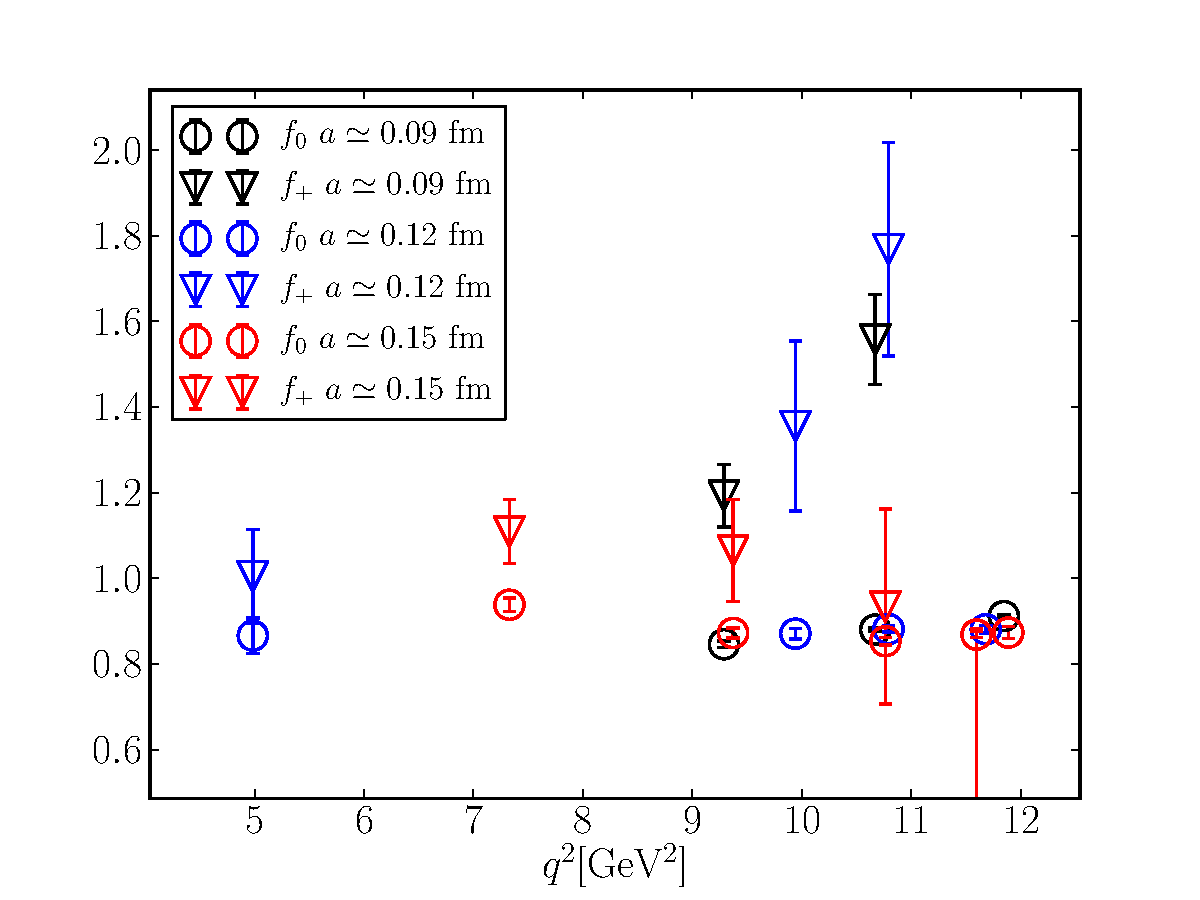
\includegraphics[width=1.0\textwidth]{images/nrqcd/BD_formfactors_fromV0S.pdf}
  \end{center}
  \caption{$B\to D$ form factors extracted from $\langle V_0 \rangle$ and $\langle S \rangle$. Clearly these results are nonsense. See text. \label{fig:f0fp_fromV0S}}
\end{figure}

Results from adopting this alternative approach (in the $B\to D$ case) is shown in Fig. \ref{fig:f0fp_fromV0S}. One immediately notices that $f_+(q^2)$ results are diverging in the $|{\textbf{p}}_{D}| \to 0$ limit. Why this occurs can be seen by inspecting Eq. \eqref{eq:fplus_badness}. For $f_+$ to remain finite, the difference between currents on the numerator must tend to zero at the same rate as ${\textbf{p}}_D^2$. Our results for the currents $\langle S \rangle$ and $\langle V_0 \rangle$ are not precise enough to produce the delicate cancellation required to accurately determine $f_+$ in the high $q^2$ region.

A quick summary of the situation. We have 3 currents, $\langle S \rangle$, $\langle V_0 \rangle$, and $\langle V_k \rangle$. We require input from two of these currents in order to determine the form factors. Large contributions to $\langle V_k \rangle$ may be being ignored, so at the moment we do not consider $\langle V_k \rangle$ a 'trustworthy' estimation of the continuum spacial vector current. Using only $\langle S \rangle$ and $\langle V_0 \rangle$ leads to a divergence of $f_+(q^2)$ as $q^2\to q^2_{\text{max}}$, so is also untenable. In the next section, we show an approach we attempted to finding new normalizations of these three currents such that all three can be 'trusted' as good approximations to the continuum current. One could then in principle use these trustworthy $\langle V_0 \rangle$ and $\langle V_k \rangle$ currents to extract the form factors.

\section{Non-Perturbative Renormalization using $B_c\to \eta_c$ Data}
\label{sec:Bcetac}

Here we define non-perturbative normalization constants $Z_J$ for the NRQCD-HISQ currents via 
\begin{align}
  \nonumber
	J &= ( 1 + z^J_0 \alpha_s )( J^{(0)} + J^{(1)} ) + \mathcal{O}(\, \alpha_s^2, \, (\Lambda_{\text{QCD}}/m_b)^2, \, ({\textbf{p}}/m_b)^2,\,\,\alpha_s \Lambda_{\text{QCD}} / m_b,\, \alpha_s {\textbf{p}}/m_b ) \\
	&\equiv Z_{J}( 1 + z^J_0 \alpha_s )( J^{(0)} + J^{(1)} ), \\ \nonumber &\quad\quad Z_{J} = 1 +  \mathcal{O}(\, \alpha_s^2, \, (\Lambda_{\text{QCD}}/m_b)^2, \, ({\textbf{p}}/m_b)^2,\,\,\alpha_s \Lambda_{\text{QCD}} / m_b,\, \alpha_s {\textbf{p}}/m_b ).
	\label{eq:overall}
\end{align}
The $Z_J$ factor compensates for the truncation of the series. One can imagine fixing $Z_J$ by demanding some property of $J$. One may be concerned that $Z_J$ is dependent on the spacial momenta in the current $Z_J=Z_J({\textbf{p}})$, however, we will see below that this variation is a negligable effect.

In this section, we outline an approach used to determine $Z_S$, $Z_{V_0}$ and $Z_{V_k}$. In this process we use NRQCD data from another HPQCD project of determining form factors for $B_c \to \eta_c l\nu$ decays \cite{Colquhoun:2016osw}. A schematic of how this is achieved is given in fig. \ref{fig:normalization_chain}. I thank Brian Colquhoun for supplying correlation functions from their calculation. The current in this calculation is the same as in the $B_{(s)}\to D_{(s)}l\nu$ calculation, so normalizations determined using this data can in principle be applied to the $B_{(s)}\to D_{(s)}l\nu$ calculation.

\begin{figure}[htb!]
\hspace{-5pt}
    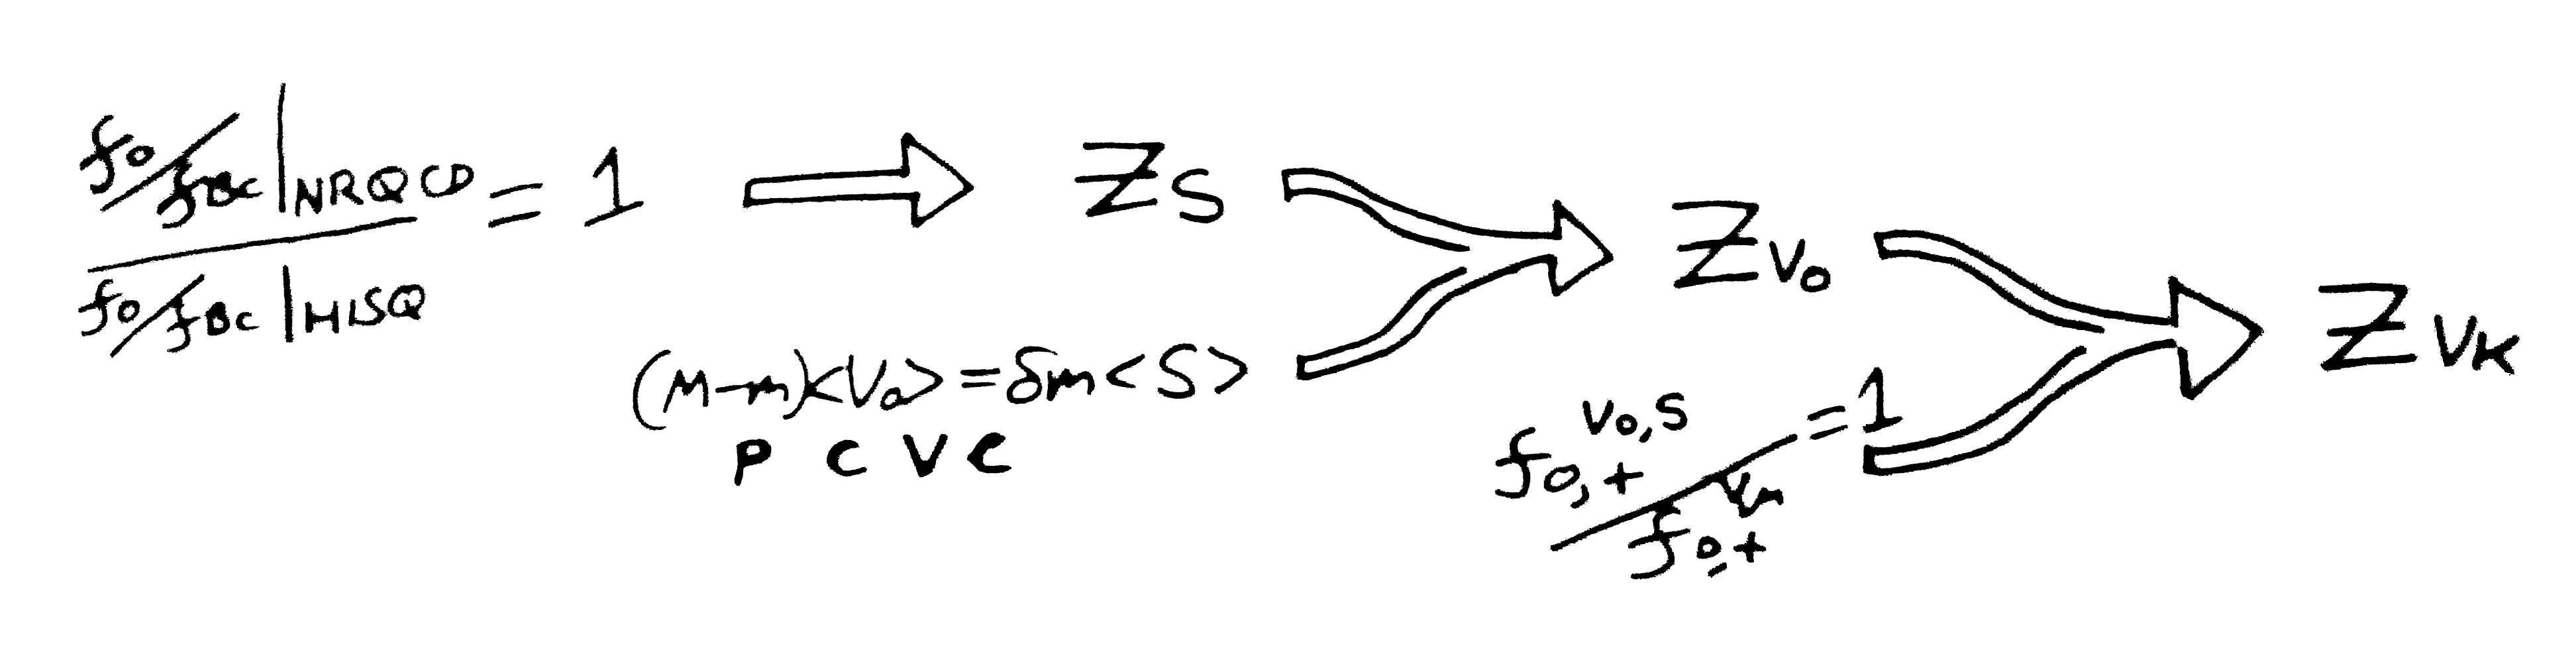
\includegraphics[width=1.0\textwidth]{images/nrqcd/normalization_chain.jpg}
  \caption{A schematic of the chain of steps towards normalizing the scalar, temporal vector and spacial vector NRQCD-HISQ currents. Details given in the next three sections; \ref{sec:Zs}, \ref{sec:ZV0} and \ref{sec:ZVk}. \label{fig:normalization_chain}}
\end{figure}

We use the $B_c \to \eta_c l\nu$ data here since
\begin{itemize}
\item
  $B_c\to \eta_c$ correlators have much smaller statistical errors. This is because of the lack of the $s$ spectator quark, degradation of the signal/noise ratio is less severe (see Sec. \ref{sec:signaldegredation}).
\item
  A heavy-HISQ determination of $B_c\to \eta_c$ form factors was also available from their project \cite{Colquhoun:2016osw}. This comes in useful in our approach to the normalization.
\end{itemize}
All analysis below is performed using data on the fine ensemble (set 2). In principle, it could be repeated for any other ensemble on which correlators for any $b\to c$ transition is available.

\subsection{$Z_S$}
\label{sec:Zs}

We have avaliable to us lattice results for $f_0^{B_c\to \eta_c}(q^2)\equiv f_0(q^2)$ for a number of $q^2$ values spanning the entire $q^2$ range (including $q^2_{\text{max}}$ and $q^2=0$) from the NRQCD-HISQ $S$ current on the fine ensemble. We also have a determination of $f_{B_c}$ also from NRQCD-HISQ lattice currents on the same ensemble. We denote these finite-$a$ lattice results as $\hat{f}_0(q^2)$, $\hat{f}_{B_c}$. We also have a continuum-extrapolated heavy-HISQ result for $f_0(q^2)/f_{B_c}$, for $q^2_{\text{max}}$ and $q^2=0$. This is given in the form of this ratio since discretization effects largely cancel in this ratio improving the continuum extrapolation (see Chapters \ref{chap:BsDsstar} and \ref{chap:BsDs}). The results are
\begin{align}
  {f_0(q^2_{\text{max}})\over f_{B_c}} = 2.104(36),\quad {f_0(0)\over f_{B_c}} = 1.288(42).
\end{align}
Since $f_0\propto \langle S \rangle$, we can assert that $f_0 = Z_S \hat{f}_0$, i.e., the continuum $f_0$ contains the normalization that $\hat{f}_0$ is missing. Similarly for $\hat{f}_{B_c}$ and $Z_{A_0}$. Hence by demanding that the NRQCD-HISQ finite-$a$ results match the continuum heavy-HISQ results, we can find, for example
\begin{align}
  {Z_S \over Z_{A_0}}\bigg\vert_{q^2_{\text{max}}} = {f_0(q^2_{\text{max}})/f_{B_c}\over \hat{f}_0(q^2_{\text{max}})/\hat{f}_{B_c}} = 0.995(15).
\end{align}
As a test to see if $Z_S$ varies with ${\textbf{p}}$, we can compare this result to an analagous approach at $q^2=0$;
\begin{align}
  {Z_S \over Z_{A_0}}\bigg\vert_{q^2=0} = {f_0(0)/f_{B_c}\over \hat{f}_0(0)/\hat{f}_{B_c}} = 0.962(33).
\end{align}
A similar approach cannot be applied for $Z_{V_0}$ or $Z_{V_k}$, since $f_0$ has a complicated relationship to both $\langle V_0 \rangle$ and $\langle V_k \rangle$ that varies with $q^2$, so it is not clear how one attribute discrepancies between $\hat{f}_0/\hat{f}_{B_c}$ and $f_0/f_{B_c}$ to $Z_{V_0}$ and $Z_{V_k}$.

The comparison of these two ratios at $q^2_{\text{max}}$ and $q^2=0$ show that any variation is small in comparison to statistical errors. We can absorb the variation in ${\textbf{p}}$ into a subleading term in the scalar current by demanding that $Z_{S}/Z_{A_0}|_{q^2_{\text{max}}} = Z_{S}/Z_{A_0}|_{q^2=0}$. Redefine the scalar current according to:
\begin{align}
 S = Z_{S} \left[ (1 + z^{S}_0 \alpha_s)( V_0^{(0)} - V_0^{(1)} ) + \alpha_s z^{S}_2 V_0^{(2)} \right].
\end{align}
We can determine $z_2^S$ by demanding that $Z_S$ does not vary between $q^2_{\text{max}}$ and $q^2=0$. This is equivilant to the $V_0^{(2)}$ term absorbing all of the variation in the normalization on ${\textbf{p}}$, which one would expect since this current is proportional to the spacial momentum in the $c$-quark.

By defining $\hat{f}_2$ to be $\hat{f}_0$ but with $(1+\alpha_s z_0^S)( V_0^{(0)} - V_0^{(1)} )$ replaced with $\alpha_s V_0^{(2)}$, we can write:
\begin{align}
	{Z_{A_0}\over Z_{S}} = { ( \hat{f}_0 + z^S_2 \hat{f}_2 )/ \hat{f}_{B_c}  \over f_0/f_{B_c} } \equiv \left({Z_{A_0}\over Z_{S}}\right)^{(0,1)} + z^S_2 \left({Z_{A_0}\over Z_{S}}\right)^{(2)}.
\end{align}
With this further definition, and demanding that ${Z_{A_0}/ Z_{S}}|_{q^2_{\text{max}}} = {Z_{A_0}/ Z_{S}}|_{q^2=0}$, we end up with
\begin{align}
	z^S_2 = { \left({Z_{A_0}\over Z_{S}}\right)^{(0,1)}\big\vert_{q^2=0} - \left({Z_{A_0}\over Z_{S}}\right)^{(0,1)}\big\vert_{q^2_{\text{max}}}
\over \left({Z_{A_0}\over Z_{S}}\right)^{(2)}\big\vert_{q^2_{\text{max}}} - \left({Z_{A_0}\over Z_{S}}\right)^{(2)}\big\vert_{q^2=0} }
 = -1.1(1.5).
\end{align}
Now that we are able to include $V_0^{(2)}$ in the scalar current, we can consider the scalar current normalized up to $\mathcal{O}(\alpha_s^2, \,(\Lambda_{\text{QCD}}/m_b)^2, \,({\textbf{p}}/m_b)^2, \alpha_s\Lambda_{\text{QCD}}/m_b )$. We can use
\begin{align}
  S = (1+z_0^S\alpha_s)( V_0^{(0)} - V_0^{(1)} ) + z_2^s\alpha_s V_0^{(2)} + \mathcal{O}(\alpha_s^2, \,(\Lambda_{\text{QCD}}/m_b)^2, \,({\textbf{p}}/m_b)^2,\,\, \alpha_s\Lambda_{\text{QCD}}/m_b )
\end{align}
(Yes, we have not strictly determined $Z_S$ in this case, but we will for the vector currents). The next steps are essentially to match results using the vector currents to this newly normalized scalar current, meaning the vector currents will be normalized up to $\mathcal{O}(\alpha_s^2, \,(\Lambda_{\text{QCD}}/m_b)^2, \,({\textbf{p}}/m_b)^2 \,,\,\, \alpha_s\Lambda_{\text{QCD}}/m_b)$, hence we then will have theoretically accounted for the large subleading pieces in the spacial vector current, since we have accounted for $\alpha_s{\textbf{p}}/m_b$ order terms.

\subsection{$Z_{V_0}$}
\label{sec:ZV0}

We normalize the temporal vector current via its PCVC relation with the now 'correctly' normalized scalar current.

This also has the benefit of partially removing the $f_+(q^2)$ divergence as ${\textbf{p}}^2_{\eta_c}\to 0$ when extracted from $\langle V_0 \rangle$ and $\langle S \rangle$. We can see this by inspecting the expression for $f_+(q^2)$ in terms of $\langle S \rangle$ and $\langle V_0 \rangle$(Eq. \eqref{eq:fplus_badness}). As ${\textbf{p}}_{\eta_c}^2 \to 0$ the numerator becomes proportional to $\delta m \langle S \rangle - (M_{B_c}-M_{\eta_c}) \langle V_0 \rangle$, which vanishes when the PCVC relation is satisfied. So one would expect if we renormalize one of the currents so the Ward identity is satisfied (at $q^2_{\text{max}}$), this divergence should be removed or at least reduced.

\begin{figure}[htb!]
\centering
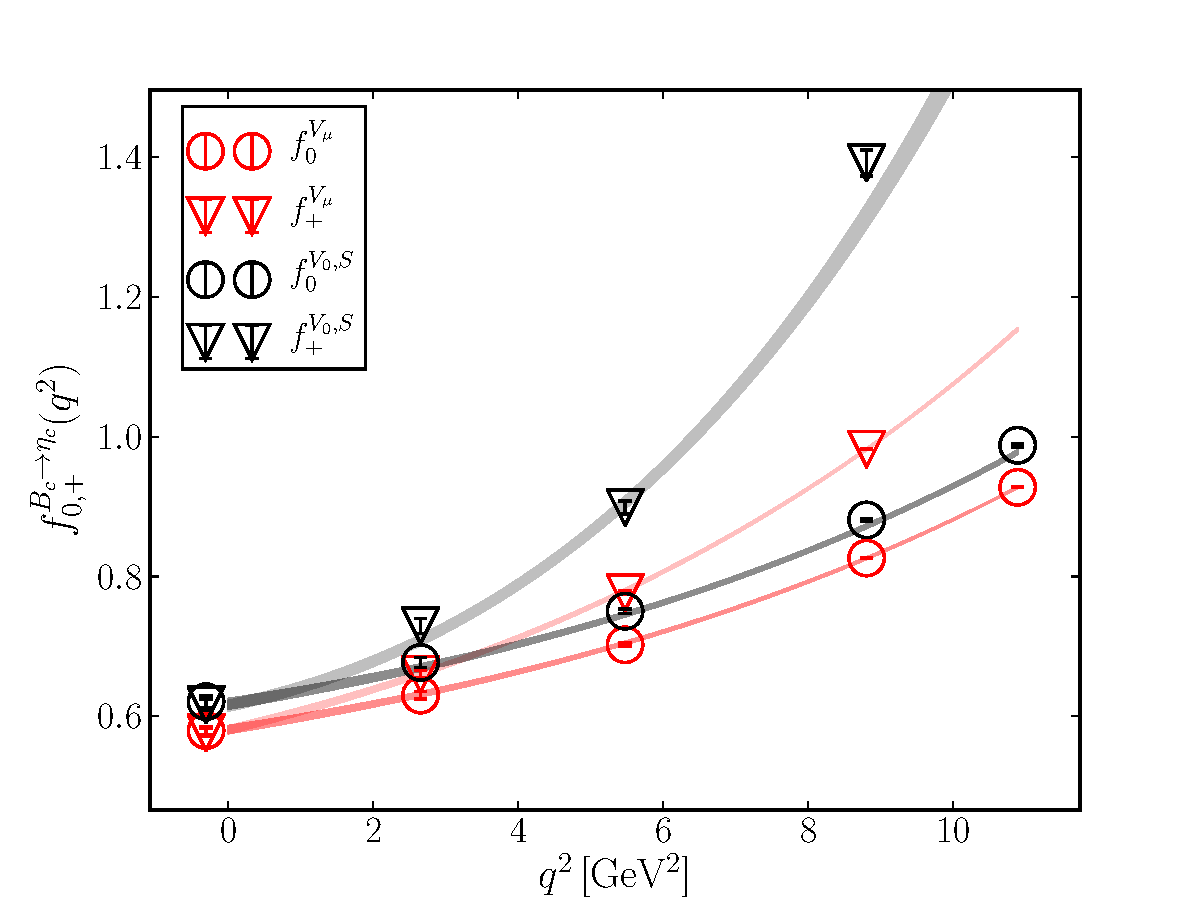
\includegraphics[scale=0.55]{images/nrqcd/Bcetac_bothways_1.pdf}
\caption{Comparison of form factors from $\langle V_0 \rangle, \langle S \rangle$ and $\langle V_0 \rangle,\langle V_k \rangle$, no additional normalizations. The bands show the resuls of fitting the data to the BGL parameterization \eqref{eq:zexpansion}, where coefficients $a^{0,+}_n$ are fit parameters. These bands are intended simply to guide the eye. \label{fig:naive}}
\end{figure}

Hence we should normalize the temporal vector current using the already normalized scalar density. So to satisfy the PCVC, Multiply $\langle V_0 \rangle$ by 
\begin{align}
	Z_{V_0} = {m_b-m_c \over M_{B_c}-M_{\eta_c} } { \langle S \rangle \over \langle V_0 \rangle }\Big\vert_{q^2_{\text{max}}} = 1.0661(36).
	\label{eq:Zward}
\end{align}
This seems to deal with the $f_+$ divergence. Fig. \ref{fig:naive} compares form factors determined using $\langle V_0 \rangle$, $\langle S \rangle$, and $\langle V_0 \rangle$, $\langle V_k \rangle$, {\textit{before}} imposing $Z_{V_0}$, and Fig. \ref{fig:Zward} shows the same {\textit{after}} $\langle V_0 \rangle$ has been multiplied by $Z_{V_0}$.
\begin{figure}[htb!]
\centering
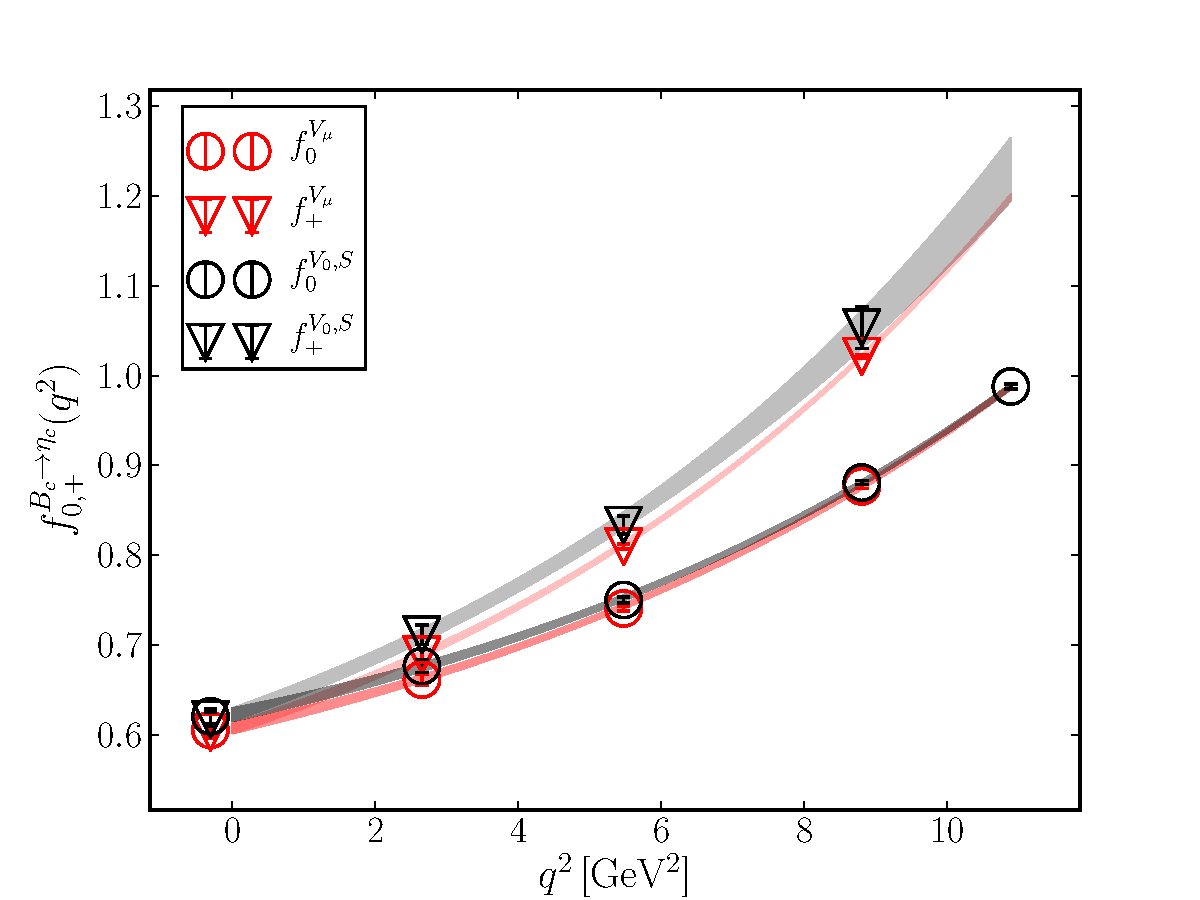
\includegraphics[scale=0.55]{images/nrqcd/Bcetac_bothways_2.pdf}
\caption{Comparison of form factors from $\langle V_0 \rangle,\langle S \rangle $ and $\langle V_0\rangle,\langle V_k\rangle$, $\langle V_0\rangle$ is mutliplied by $Z_{V_0}$ given in \eqref{eq:Zward}. The bands show the resuls of fitting the data to the BGL parameterization \eqref{eq:zexpansion}, where coefficients $a^{0,+}_n$ are fit parameters. \label{fig:Zward}}
\end{figure}

Unfortunately the same technique does not solve the diverging $f_+$ issue in the $B_{(s)}\to D_{(s)}$ case, the statistics are not as good so the divergence is too severe. 

\subsection{$Z_{V_k}$}
\label{sec:ZVk}

We can determine a $Z_{V_k}$ by demanding that $f_{0,+}^{V_0,S}/f_{0,+}^{V_{\mu}}=1$, with the knowledge that $\langle V_0 \rangle, \langle S \rangle$ require no further normalization. This can be done with both $f_+$ and $f_0$, at any $q^2$;
\begin{align}
	Z_{V_k} &= 1 + {f_+^{V_0,S} - f_+^{V_{\mu}} \over R_{+k} \langle V_k \rangle }  \\
	&= 1 + {f_0^{V_0,S} - f_0^{V_{\mu}} \over R_{0k} \langle V_k \rangle },
\end{align}
where the $R$'s are some kinematic gunk: $R_{+k} = ( M_{B_c} - E_{\eta_c} )/2M_{B_c}{\textbf{p}}_{\eta_c}/\sqrt{3}$, \\ $R_{0k} = R_{+k} - {( M_{B_c}^2-M_{\eta_c}^2 )(M_{B_c}-E_{\eta_c})/2M_{B_c} {\textbf{p}}_{\eta_c}/q^2\sqrt{3}}$. The results are shown in Fig. \ref{fig:ZVk}.
\begin{figure}[htb!]
\centering
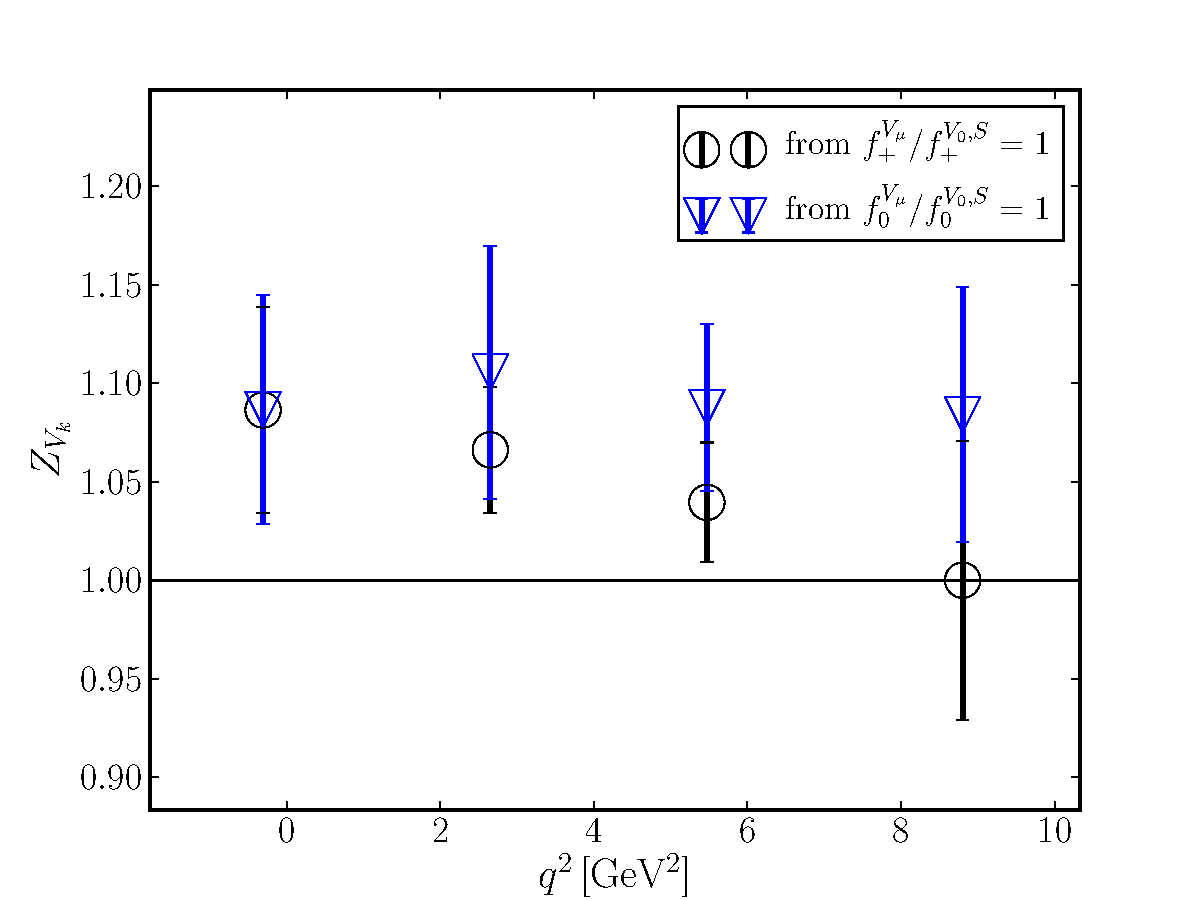
\includegraphics[scale=0.5]{images/nrqcd/ZVk.pdf}
\caption{$Z_{V_k}$ from constraining form factors to be the same from $\langle V_0 \rangle,\langle S \rangle$ and $\langle V_0 \rangle,\langle V_k \rangle$}
\label{fig:ZVk}
\end{figure}
The fact that these are not varying by a statistically significant extent in $q^2$ implies that the spacial vector normalization does not vary strongly in ${\textbf{p}}_{\eta_c}$. Hence, since these are all estimates of the same value, we can average over them to get
\begin{align}
	Z_{V_k} = 1.070(36).
\end{align}
When this normalization is given to $\langle V_k \rangle$, the $B_c\to\eta_c$ form factors from the two methods become consistent, see Fig. \ref{fig:identicle}.

\begin{figure}[htb!]
\centering
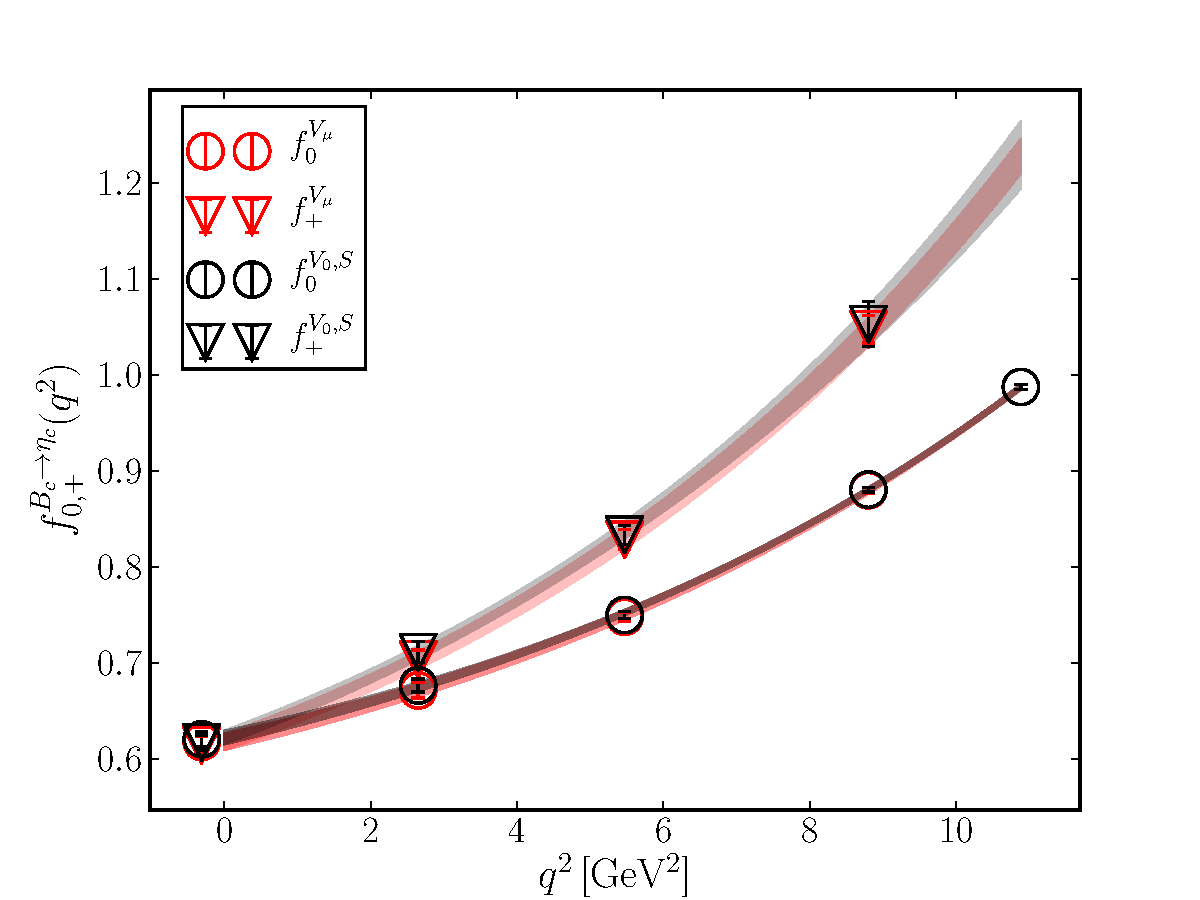
\includegraphics[scale=0.55]{images/nrqcd/Bcetac_bothways_3.pdf}
\caption{Comparison of form factors from $\langle V_0 \rangle, \langle S \rangle$ and $\langle V_0 \rangle,\langle V_k \rangle$, with $\langle V_0 \rangle$ normalized with $Z_{V_0}$ and $\langle V_k \rangle$ normalized with $Z_{V_k}$. The bands show the resuls of fitting the data to the BGL parameterization \eqref{eq:zexpansion}, where coefficients $a^{0,+}_n$ are fit parameters. \label{fig:identicle}}
\end{figure}

One could imagine using these normalizations $Z_{V_0}$ and $Z_{V_k}$ in the $B_{(s)}\to D_{(s)}$ calculation. The errors of this normalization are around $4\%$, which would push the final results of the $B_{(s)}\to D_{(s)}$ study up to the $5-10\%$ range. At present this level of precision is not competitive in comparison to other calculations of these quantities.

If one choses to trust the normalization of the scalar current, this analysis shows that (on the fine ensemble) the extra normalization required for the vector currents beyond what is usually implemented is a large effect ($Z_{V_0}-1\sim Z_{V_k}-1\sim 7\%$). This would suggest that the currently used truncation of the NRQCD-HISQ vector current is missing $\sim 7\%$ from the neglected terms lower down in the series. 

\section{Conclusion of NRQCD work}

As mentioned in the introduction - the main takehome of this thesis is that using NRQCD (namely NRQCD-HISQ currents) to compute form factors for $b\to c$ transitions, is far from optimal. 

We rely here on truncations in many different interlocking series ($1/m_b, \alpha_s,\alpha_s/m_b,...$), which may leave out important information. The terms in the series we {\textit{do}} have access to rely on perturbation theory via the matching factors. Some progress was made to normalize currents non-perturbatively in the above work, but our results fall short of what would be required to obtain precise continuum results.

I hope that in reading this chapter you experienced a similar feeling of confusion and anxiety to what I felt as I carried out this work. It was only after many months of grappling with the problems of these calculations that we decided to put them aside and attempt instead the heavy-HISQ approach from scratch. Reading the following two chapters, both dedicated to successful heavy-HISQ studies, will feel like a warm bath in comparison to the NRQCD experience. The heavy-HISQ approach is in contrast very elegant, contains far less assumptions, and results in cleaner signals.
